\documentclass[12pt]{article}

\usepackage{multirow}
\usepackage{amsmath}
\usepackage{amsfonts}
\usepackage{float}
\usepackage{fancyhdr}
\usepackage{graphicx}
\usepackage{setspace}
\usepackage{subcaption}
\usepackage{booktabs}
\usepackage{bm}
\usepackage[colorlinks=true,linkcolor=blue, citecolor=red]{hyperref}
\usepackage{url}
\usepackage[top=.75in, left=.75in, right=.75in, bottom=1in]{geometry}
\usepackage[utf8]{vietnam}

% For algorithm
\usepackage{mathtools}
\usepackage{algorithm}
 \usepackage[noend]{algpseudocode}
 \usepackage{setspace, etoolbox, caption}

\usepackage{algpseudocode}


% ============ CODE ============
\usepackage{listingsutf8}%\usepackage{listings}
\usepackage{xcolor}
\definecolor{codegreen}{rgb}{0,0.6,0}
\definecolor{codegray}{rgb}{0.5,0.5,0.5}
\definecolor{codepurple}{rgb}{0.58,0,0.82}
\definecolor{backcolour}{rgb}{0.95,0.95,0.92}

% Styling for the code.
\lstdefinestyle{mystyle}{
    backgroundcolor=\color{backcolour},   
    commentstyle=\color{codegreen},
    keywordstyle=\color{magenta},
    numberstyle=\tiny\color{codegray},
    stringstyle=\color{codepurple},
    basicstyle=\ttfamily\footnotesize,
    breakatwhitespace=false,         
    breaklines=true,                 
    captionpos=b,                    
    keepspaces=true,                 
    numbers=left,                    
    numbersep=5pt,                  
    showspaces=false,                
    showstringspaces=false,
    showtabs=false,                  
    tabsize=2
}
\lstset{style=mystyle}

% Disable indentation on new paragraphs
%\setlength{\parindent}{0pt}

% Line spacing 1.5
\renewcommand{\baselinestretch}{1}

% Optional: graphic path
% \graphicspath{PATH_TO_GRAPHIC_FOLDER}

% To use Times font family, uncomment this row
% \usepackage{mathptmx}

% To use roman section / subsection, uncomment these rows
% \renewcommand{\thesection}{\Roman{section}}
% \renewcommand{\thesubsection}{\thesection.\Roman{subsection}}

% Define course name, report name and report title.
\newcommand{\coursename}{Phương pháp toán cho Trí tuệ nhân tạo}
\newcommand{\reportname}{Dự đoán giá xe bằng mô hình Linear Regression}
\newcommand{\reporttitle}{Báo cáo Lab 1}

\newcommand{\studentname}{Nguyễn Đình Hà Dương (23122002)\\Nguyễn Lê Hoàng Trung (23122004)\\Đinh Đức Tài (23122013)\\Hoàng Minh Trung (23122014)}
\newcommand{\teachername}{TS. Cấn Trần Thành Trung\\ThS. Nguyễn Ngọc Toàn}

\newcommand{\leftfooter}{\LaTeX\ by \href{https://github.com/ductai05}{Duc Tai Dinh}}

% ============ HEADER AND FOOTER ============
% Header length
\setlength{\headheight}{29.43912pt}

% Footer page number would be on the lower-right corner
\pagestyle{fancy}
\fancyfoot{}
\fancyfoot[R]{Trang \thepage}

\lhead{Lab 1: Dự đoán giá xe}
\rhead{
Trường Đại học Khoa học Tự nhiên - ĐHQG HCM\\
\coursename
}
\lfoot{\leftfooter}

% ============ DOCUMENT ============
\begin{document}
\begin{titlepage}
\newcommand{\HRule}{\rule{\linewidth}{0.5mm}}
\centering

\textsc{\LARGE đại học quốc gia tphcm}\\[1.5cm]
\textsc{\Large trường đại học khoa học tự nhiên}\\[0.5cm]
\textsc{\large khoa công nghệ thông tin}\\[0.5cm]
\textsc{AI23 (23TNT1), FIT@HCMUS-VNUHCM}\\[0.5cm]

\HRule \\[0.4cm]
{ 
\huge{\bfseries{\reporttitle}}\\[0.5cm]
\large{\bfseries{Đề tài: \reportname}}
}\\[0.4cm]
\HRule \\[0.5cm]

\textbf{\large Môn học: \coursename}\\[0.5cm]

\begin{minipage}[t]{0.5\textwidth}
\begin{flushleft} \large
\emph{Sinh viên thực hiện:}\\
\studentname
\end{flushleft}
\end{minipage}
~
\begin{minipage}[t]{0.4\textwidth}
\begin{flushright} \large
\emph{Giáo viên hướng dẫn:} \\
\teachername
\end{flushright}
\end{minipage}\\[1.5cm]

{\large \today}\\[0.5cm]


\includegraphics[scale=.3]{img/hcmus-logo.png}\\[1cm] 

\vfill
\end{titlepage}
	
	
\tableofcontents
\pagebreak

\newpage
\section{Giới thiệu}

\paragraph{}{Đây là bài báo cáo cho \textbf{Lab 1 - Dự đoán giá xe}, môn Phương pháp toán cho Trí tuệ nhân tạo, lớp Trí tuệ nhân tạo Khóa 2023 (23TNT1), Khoa Công nghệ thông tin, Trường Đại học Khoa học tự nhiên - Đại học Quốc gia TP.HCM. Trong bài báo cáo này, chúng tôi sẽ trình bày phương pháp \textbf{dự đoán giá xe} bằng \textbf{mô hình hồi quy tuyến tính} dựa trên dữ liệu huấn luyện được cho trước.}

\paragraph{}{\textbf{Báo cáo được thực hiện bởi nhóm các thành viên:}} 
\begin{itemize}
    \item Nguyễn Đình Hà Dương (23122002)
    \item Nguyễn Lê Hoàng Trung (23122004)
    \item Đinh Đức Tài (23122013)
    \item Hoàng Minh Trung (23122014)
\end{itemize}

\paragraph{}{\textbf{Đường dẫn repository Github của báo cáo:}} \href{https://github.com/ductai05/Math-For-AI}{https://github.com/ductai05/Math-For-AI} \cite{repo}

\paragraph{}{\textbf{Bảng phân công nhiệm vụ cho từng thành viên:}}

\begin{table}[H]
\centering
\renewcommand{\arraystretch}{1.4}
\label{tab:phancongnv}
\begin{tabular}{|c|c|l|}
\hline
\textbf{Họ và tên} & \textbf{MSSV} & \multicolumn{1}{c|}{\textbf{Nhiệm vụ}} \\ \hline
\begin{tabular}[c]{@{}c@{}}Nguyễn Đình \\ Hà Dương\end{tabular} &
  23122002 &
  \begin{tabular}[c]{@{}l@{}}- Linear regression với phương pháp PCA.\\ - Cơ sở toán học của Linear regression \& Ridge regression \& PCA.\end{tabular} \\ \hline
\begin{tabular}[c]{@{}c@{}}Nguyễn Lê \\ Hoàng Trung\end{tabular} &
  23122004 &
  \begin{tabular}[c]{@{}l@{}}- Polynomial linear regression.\\ - Cơ sở toán học của Polynomial linear regression. Code testing.\end{tabular} \\ \hline
\begin{tabular}[c]{@{}c@{}}Đinh \\ Đức Tài\end{tabular} &
  23122013 &
  \begin{tabular}[c]{@{}l@{}}- Data preprocessing, visualization, encoding, normalization.\\ - Simple linear regression \& Evaluation metrics. Review report.\end{tabular} \\ \hline
\begin{tabular}[c]{@{}c@{}}Hoàng \\ Minh Trung\end{tabular} &
  23122014 &
  \begin{tabular}[c]{@{}l@{}}- Multiple linear regression \\ - Cơ sở toán học của Multiple linear regression \& Lasso regression\end{tabular} \\ \hline
\end{tabular}
\end{table}

\paragraph{}{\textbf{Các thư viện và công nghệ sử dụng:}}

\begin{itemize}
    \item Numpy: thư viện Python để xử lý số học.
    \item Pandas: thư viện Python để thao tác và xử lý dữ liệu.
    \item Matplotlib: thư viện Python để trực quan hóa dữ liệu.
    \item Jupyter Notebook (thông qua jupyter, ipykernel): Môi trường làm việc tương tác cho phép kết hợp mã thực thi, văn bản mô tả (Markdown), công thức toán học và trực quan hóa trong cùng một tài liệu.
    \item Visual Studio Code: Trình soạn thảo mã nguồn (IDE). 
    \item Git, Github: Quản lý dự án, lưu và chia sẻ source code.
\end{itemize}

\pagebreak % nhiem vu
\newpage
\section{Nền tảng toán học}

\paragraph{}{Các kiến thức trong phần này được trích dẫn từ sách Giáo trình bài tập Xác suất thống kê \cite{xstk}, trường Đại học Khoa học tự nhiên, ĐHQG-HCM và một số trang thông tin khác.}

\subsection{Chuẩn hóa Z-score}
\label{label:standart scaler}

\paragraph{}{\textbf{Chuẩn hóa Z-score} là phương pháp biến đổi dữ liệu có phân phối chuẩn bất kì về phân phối chuẩn hóa.} Tức là, nếu \(u\) là giá trị chuẩn hóa của dữ liệu ban đầu thì \textbf{\(u \sim N(0,1)\)}.

\paragraph{}{Dữ liệu sau quá trình chuẩn hóa thường được gọi là dữ liệu chuẩn hóa hoặc \textbf{điểm Z (Z-scores)}. Giá trị của Z-score thường nằm trong khoảng \([-3, 3]\).}

\paragraph{}{\textbf{Công thức chuẩn hóa đối với tổng thể:} Nếu một biến ngẫu nhiên $X$ tuân theo phân phối chuẩn (tức là $X \sim N(\mu, \sigma^2)$), thì điểm Z được tính bằng công thức:}
\[
Z = \frac{X - \mu}{\sigma}
\]
\paragraph{}{Trong đó:}
\begin{itemize}
    \item $Z$: Điểm Z chuẩn hóa.
    \item $X$: Giá trị của biến ngẫu nhiên hoặc một giá trị cụ thể từ tổng thể.
    \item $\mu$: Trung bình của tổng thể.
    \item $\sigma$: Độ lệch chuẩn của tổng thể.
\end{itemize}

\paragraph{}{\textbf{Công thức chuẩn hóa đối với dữ liệu mẫu:}}

\paragraph{}{Trong thực tế, chúng ta thường làm việc với dữ liệu mẫu và không biết $\mu$ và $\sigma$. Khi đó, chúng ta sẽ ước lượng chúng bằng trung bình mẫu ($\bar{x}$) và độ lệch chuẩn mẫu ($s$). Điểm Z cho một giá trị cụ thể $x$ trong mẫu được tính bằng công thức:}
\[
z = \frac{x - \bar{x}}{s}
\]
\paragraph{}{Trong đó:}
\begin{itemize}
    \item $z$: Giá trị chuẩn hóa (điểm Z) của $x$ dựa trên mẫu.
    \item $x$: Giá trị dữ liệu gốc trong mẫu.
    \item $\bar{x}$: Trung bình mẫu của  dữ liệu (sample mean).
    \item $s$: Độ lệch chuẩn mẫu của dữ liệu.
\end{itemize}



\subsection{Hiệp phương sai (Covariance)}

\paragraph{}{\textbf{Hiệp phương sai} (Covariance) \cite{thongke-descriptive-statistics} là thước đo mối liên hệ tuyến tính giữa hai biến ngẫu nhiên $X$ và $Y$. Ký hiệu: $cov(X, Y)$. Hiệp phương sai giữa hai biến ngẫu nhiên $X$ và $Y$ còn được định nghĩa là kỳ vọng của tích giữa độ lệch của $X$ và $Y$ so với giá trị kỳ vọng của chúng.}

\paragraph{}{\textbf{Công thức tính hiệp phương sai:}}

\begin{center}
\large $cov(X, Y) = E[(X-E(X))(Y-E(Y))]$
\end{center}

Công thức tính trên tổng thể:
\begin{center}
\large $cov(X,Y) = \frac{1}{N} \sum_{i=1}^{N} (x_i - \mu_X)(y_i - \mu_Y)$
\end{center}

Công thức tính trên mẫu:
\begin{center}
\large $cov(X,Y) = \frac{1}{n-1} \sum_{i=1}^{n} (x_i - \bar{x})(y_i - \bar{y})$
\end{center}

Trong đó:
\begin{itemize}
    \item \( x_i, y_i \) là giá trị của quan sát thứ \(i\).
    \item \( \mu_X, \mu_Y \) là giá trị trung bình của tổng thể.
    \item \( \bar{x}, \bar{y} \) là giá trị trung bình của mẫu.
    \item \( N \) là tổng số quan sát của tổng thể.
    \item \( n \) là tổng số quan sát của mẫu.
\end{itemize}
\paragraph{}{\textbf{Trực quan bằng đồ thị:}}
\begin{figure}[H]
    \centering
    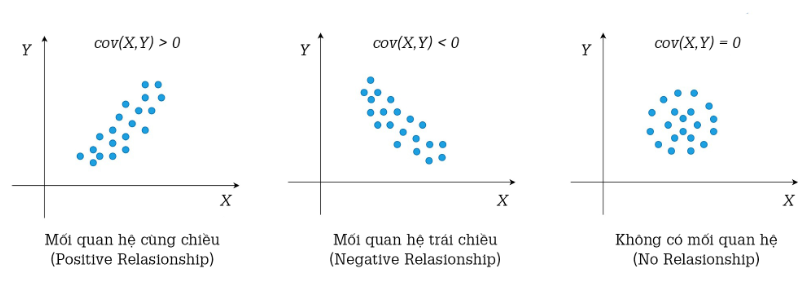
\includegraphics[width=\textwidth]{img/corvariance.png}
    \caption{Minh họa hiệp phương sai giữa hai biến ngẫu nhiên $X$ và $Y$.}
    \label{fig:covariance}
\end{figure}

\paragraph{}{Đồ thị trên minh họa ba trường hợp có thể xảy ra khi tính hiệp phương sai:}

\begin{itemize}
    \item Khi \(\text{cov}(X,Y) > 0\): Hai biến \(X\) và \(Y\) có quan hệ tuyến tính thuận, khi \(X\) tăng thì \(Y\) cũng tăng.
    \item Khi \(\text{cov}(X,Y) < 0\): Hai biến \(X\) và \(Y\) có quan hệ tuyến tính nghịch, khi \(X\) tăng thì \(Y\) giảm và ngược lại.
    \item Khi \(\text{cov}(X,Y) = 0\): Hai biến \(X\) và \(Y\) không có mối quan hệ tuyến tính với nhau.
\end{itemize}
\subsection{Ma trận hiệp phương sai (Covariance matrix)}

\paragraph{}{\textbf{Ma trận hiệp phương sai} là một ma trận vuông chứa các hiệp phương sai giữa các biến trong một tập dữ liệu. Nếu một tập dữ liệu có \( p \) biến ngẫu nhiên \( X_1, X_2, \dots, X_p \), thì ma trận hiệp phương sai \( \Sigma \) có dạng:}

\[
\Sigma =
\begin{bmatrix}
\text{Var}(X_1) & \text{Cov}(X_1, X_2) & \dots & \text{Cov}(X_1, X_p) \\
\text{Cov}(X_2, X_1) & \text{Var}(X_2) & \dots & \text{Cov}(X_2, X_p) \\
\vdots & \vdots & \ddots & \vdots \\
\text{Cov}(X_p, X_1) & \text{Cov}(X_p, X_2) & \dots & \text{Var}(X_p)
\end{bmatrix}
\]

Trong đó:
\begin{itemize}
\item \( \text{Var}(X_i) = \text{Cov}(X_i, X_i) \) là phương sai của biến \( X_i \).
\item \( \text{Cov}(X_i, X_j) \) là hiệp phương sai giữa hai biến \( X_i \) và \( X_j \).
\end{itemize}
\paragraph{}{\textbf{Công thức tổng quát:}
Giả sử có một tập dữ liệu với \( n \) quan sát và \( p \) biến ngẫu nhiên được biểu diễn dưới dạng ma trận \( X \) có kích thước \( n \times p \), với mỗi hàng là một quan sát và mỗi cột là một biến. Khi đó, ma trận hiệp phương sai được tính bằng công thức:}

\[
\Sigma = \frac{1}{n - 1} \sum_{i=1}^{n} (X_i - \bar{X})(X_i - \bar{X})^T
\]

Trong đó:
\begin{itemize}
\item \( X_i \) là vector giá trị của các biến tại quan sát thứ \( i \).
\item\( \bar{X} \) là vector trung bình của từng biến.
\end{itemize}
\paragraph{}{\textbf{Tính chất:}}
\begin{itemize}
    \item Ma trận hiệp phương sai là \textbf{ma trận đối xứng}.
    \item Đường chéo chứa phương sai của từng biến.
    \item Nếu các biến không có tương quan (độc lập tuyến tính), thì các phần tử ngoài đường chéo bằng 0.
\end{itemize}

\pagebreak
 % equation
\newpage
\section{Xử lý dữ liệu}

\subsection{Tải dữ liệu và tổng quan về dữ liệu} 
\paragraph{}{Dữ liệu phục vụ huấn luyện mô hình được cung cấp trong file \texttt{train.csv}, trong đó bao gồm:}
\begin{itemize}
    \item \textbf{1647 dòng}, cung cấp chi tiết về thông số kỹ thuật, đặc điểm và giá của các loại xe ô tô.
    \item \textbf{20 cột} dữ liệu, trong đó có 8 cột chứa dữ liệu số, 12 cột chứa dữ liệu chữ: 
    \begin{itemize}
        \item \texttt{Make}, \texttt{Model}: Hãng sản xuất xe, tên mẫu xe cụ thể.
        \item \texttt{Price}: Giá niêm yết hoặc giá bán của xe.
        \item \texttt{Year}: Năm sản xuất của xe.
        \item \texttt{Kilometer}: Tổng số kilomet xe đã di chuyển.
        \item \texttt{Fuel Type}: Loại nhiên liệu xe sử dụng (ví dụ: Xăng, Dầu Diesel, Điện).
        \item \texttt{Transmission}: Loại hộp số (ví dụ: Số sàn, Số tự động).
        \item \texttt{Location}: Địa điểm, thành phố hoặc khu vực bán xe.
        \item \texttt{Color}: Màu sơn ngoại thất của xe.
        \item \texttt{Owner}: Số lượng chủ sở hữu trước đây của xe.
        \item \texttt{Seller Type}: Loại hình người bán (ví dụ: Cá nhân, Đại lý).
        \item \texttt{Engine}: Dung tích xi-lanh của động cơ, thường tính bằng cc (cubic centimeters).
        \item \texttt{Max Power}: Công suất cực đại mà động cơ có thể tạo ra (bhp - brake horsepower).
        \item \texttt{Max Torque}: Mô-men xoắn cực đại mà động cơ có thể tạo ra (Nm - Newton-meters).
        \item \texttt{Drivetrain}: Hệ thống truyền động lực từ động cơ đến bánh xe 
        \item \texttt{Length}, \texttt{Width}, \texttt{Height}: Chiều dài, chiều rộng, chiều cao tổng thể của xe (mm).
        \item \texttt{Seating Capacity}: Số lượng chỗ ngồi tối đa trong xe (bao gồm cả lái xe).
        \item \texttt{Fuel Tank Capacity}: Dung tích tối đa của bình chứa nhiên liệu, tính bằng lít.
    \end{itemize}
    \item 149 dòng có chứa dữ liệu NaN (Not a Number).
\end{itemize}

\begin{figure}[H]
    \centering
    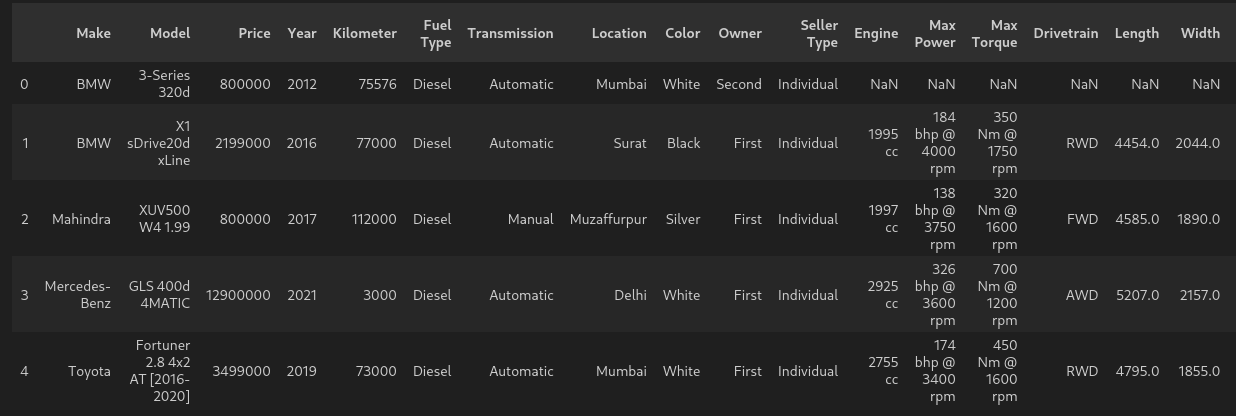
\includegraphics[width=1\linewidth]{img/data-head.png}
    \caption{Các dòng đầu tiên trong bộ dữ liệu}
    \label{fig:data-head}
\end{figure}

\subsection{Tiền xử lý dữ liệu - Data preprocessing}

\subsubsection{Chia tập dữ liệu huấn luyện - kiểm chứng}

\paragraph{}{Khi xử lí dữ liệu đầu vào, các bước như làm sạch dữ liệu và mã hóa dữ liệu sẽ lấy thông tin của tổng thể như trung vị (median), giá trị có tần suất xuất hiện lớn nhất để điền vào các dòng bị thiếu thông tin. Vì vậy, để tránh hiện tượng \textbf{rò rỉ thông tin} (data leakage), ta cần chia tập dữ liệu thành \textbf{tập huấn luyện} (training set) và \textbf{tập kiểm chứng} (validation set) ngay trước khi xử lí dữ liệu.}

\paragraph{}{Chia tập dữ liệu thành \textbf{tập huấn luyện} và \textbf{tập kiểm chứng} giúp ta đánh giá mô hình chính xác hơn, giúp nhận biết tốt hiện tượng \textbf{quá khớp} (overfitting) hoặc \textbf{dưới khớp} (underfitting).}

\paragraph{}{Tập huấn luyện và tập kiểm chứng được chia với tỉ lệ lần lượt là 0.8 và 0.2 so với tổng dữ liệu.}

\subsubsection{Làm sạch dữ liệu}
\paragraph{}{Ở bước làm sạch dữ liệu (Data cleaning), có 3 kĩ thuật chính được sử dụng:}

\begin{itemize}
    \item Điền vào ô NaN ở các cột có đặc trưng số với giá trị trung bình của chúng.
    \item Điền vào ô NaN ở các cột có đặc trưng phi số với giá trị xuất hiện thường xuyên nhất.
    \item Xóa các dòng dữ liệu lặp.
\end{itemize}

\paragraph{}{Tập kiểm chứng sẽ được điền vào ô NaN dựa trên thông tin (giá trị trung bình, giá trị xuất hiện thường xuyên nhất) lấy được từ tập huấn luyện.}

\subsubsection{Chuyển đổi dữ liệu}

\paragraph{}{Ở bước chuyển đổi dữ liệu (Data transformation), có 3 bước:}

\begin{itemize}
    \item Thêm các cột dữ liệu: \texttt{rpm at Max Power} (vòng tua tại công suất cực đại) và \texttt{rpm at Max Torque} (vòng tua tại Mô-men xoắn cực đại). 
    \item Cột dữ liệu \texttt{Max Power} và \texttt{Max Torque} được biến đổi, không còn các dữ liệu về vòng tua do đã được tách ra thành cột riêng.
    \item Các cột có đặc trưng số sẽ được đưa về dạng dữ liệu \texttt{int} (số nguyên).
\end{itemize}

\newpage
\subsection{Trực quan hóa dữ liệu - Data visualization}

\paragraph{}{Sau đây là một vài biểu đồ thể hiện chi tiết dữ liệu (trên tập train):}

\subsubsection{Ma trận tương quan của các đặc trưng số}
\begin{figure}[H]
    \centering
    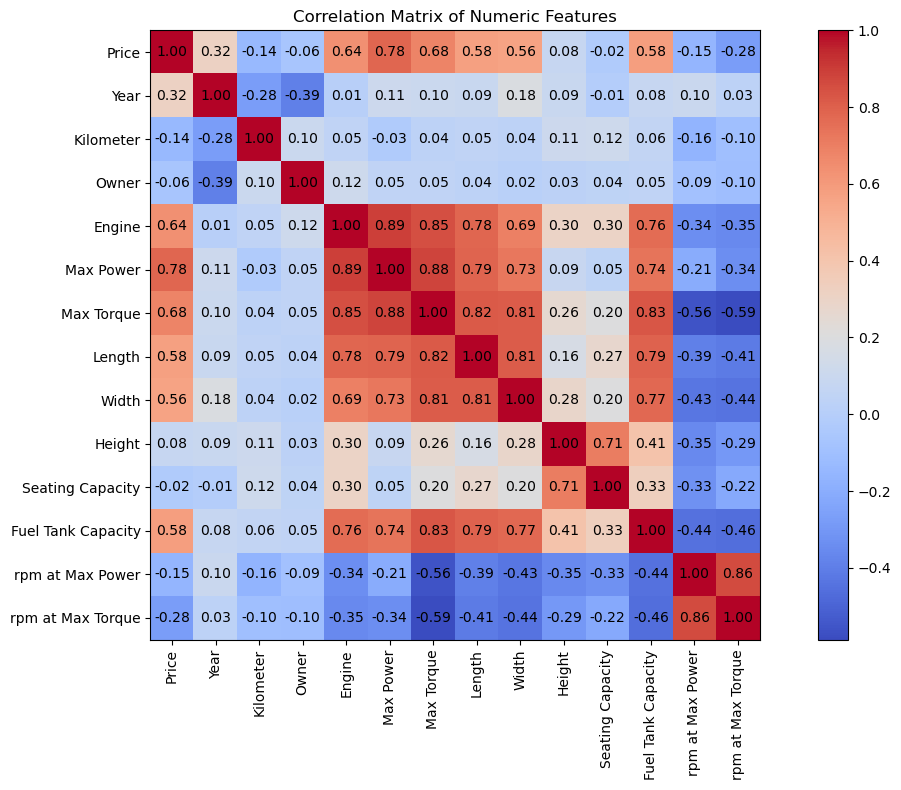
\includegraphics[width=1\linewidth]{img/corr-matrix-1.png}
    \caption{Ma trận tương quan}
    \label{fig:corr-matrix-1}
\end{figure}

\subsubsection{Biểu đồ Histogram của các đặc trưng số}
\begin{figure}[H]
    \centering
    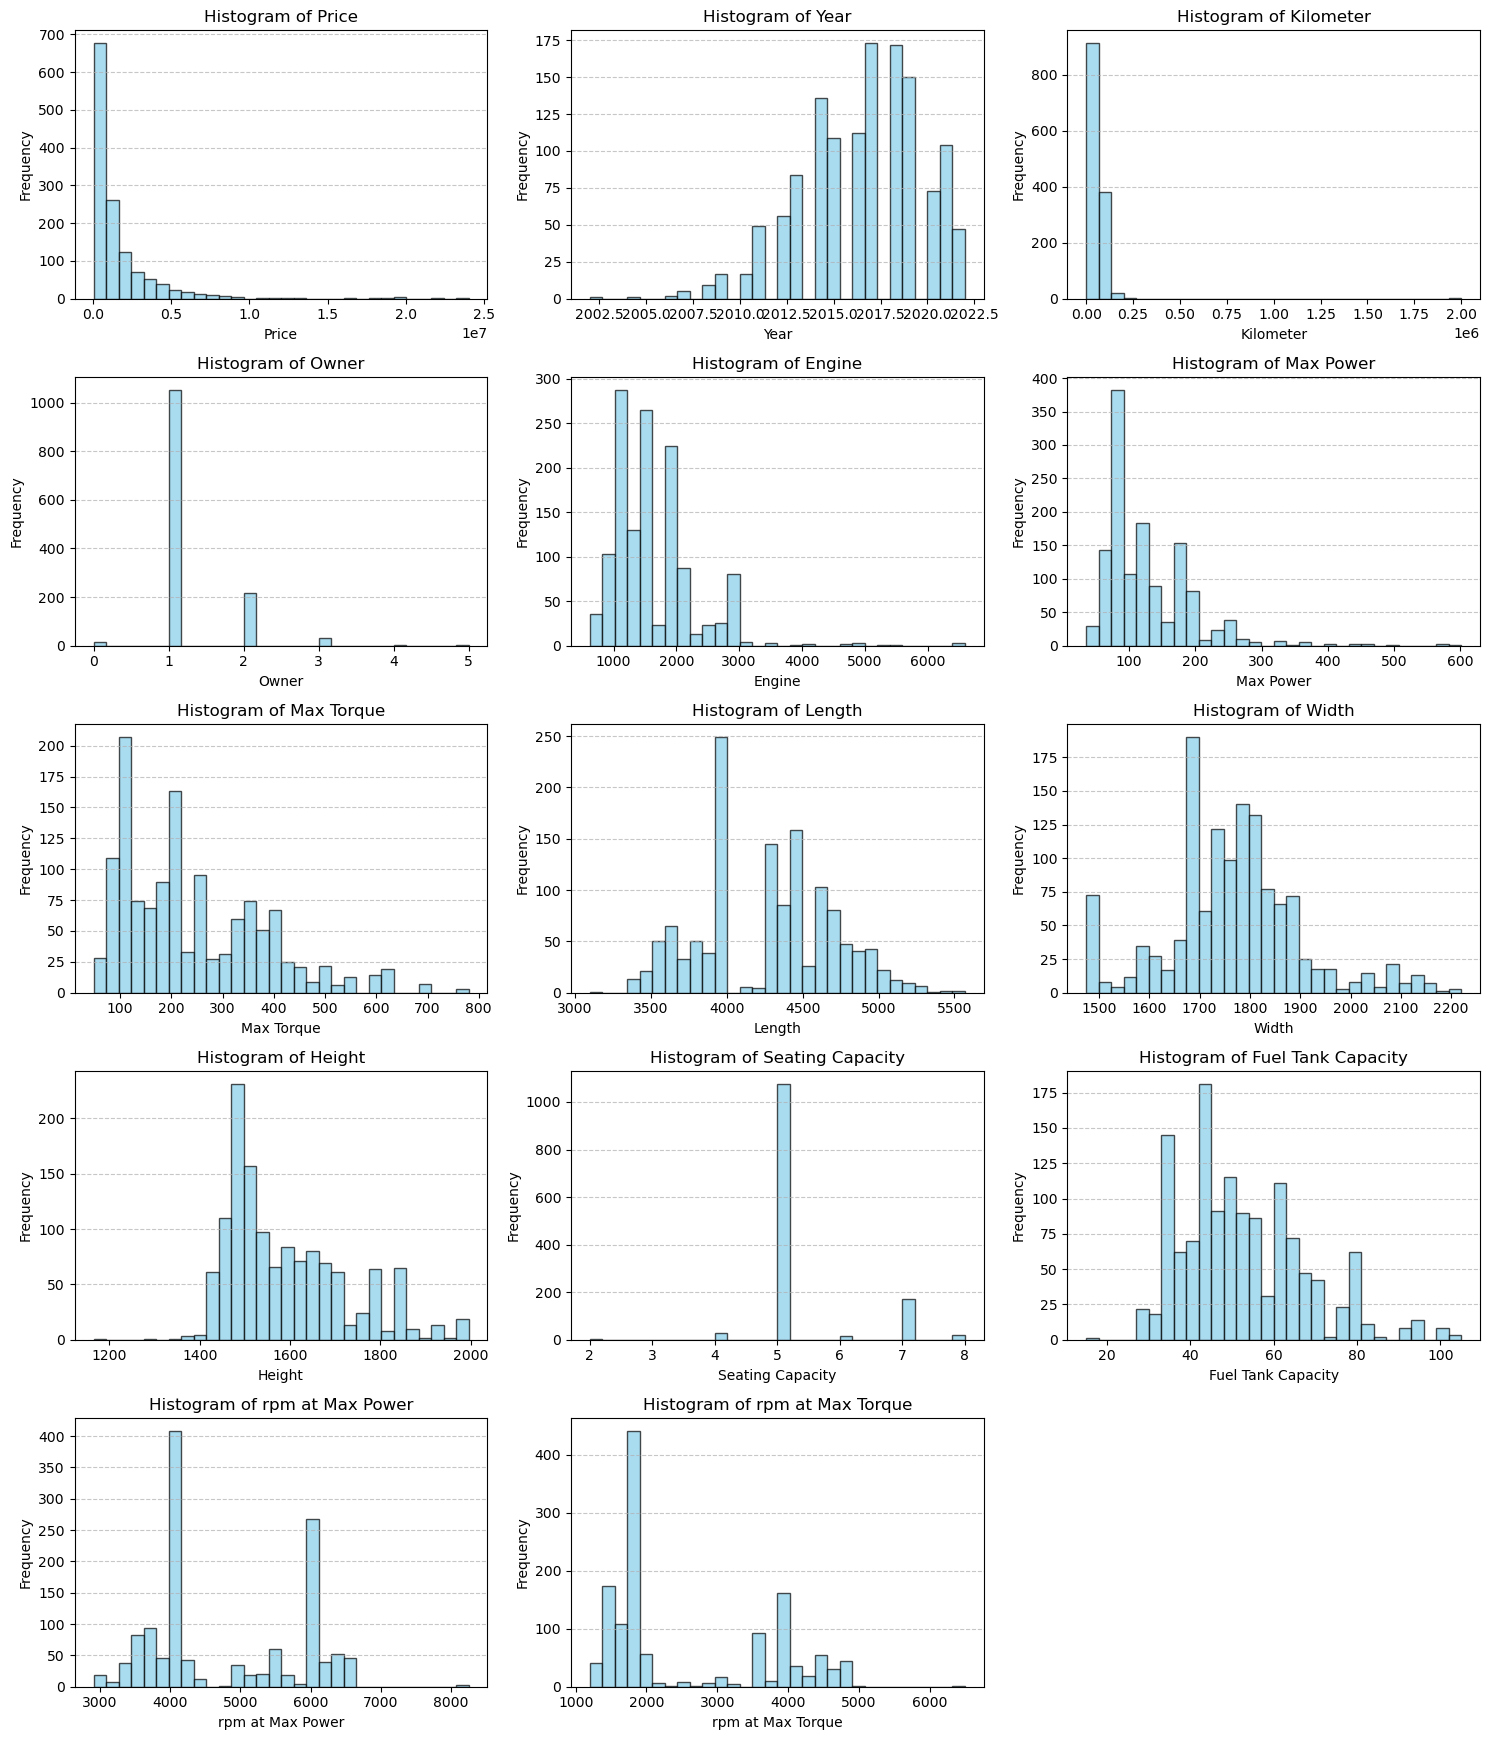
\includegraphics[width=1\linewidth]{img/histogram-1.png}
    \caption{Biểu đồ Histogram của các đặc trưng số}
    \label{fig:histogram-1}
\end{figure}

\subsubsection{Biểu đồ phân tán của các đặc trưng số}
\begin{figure}[H]
    \centering
    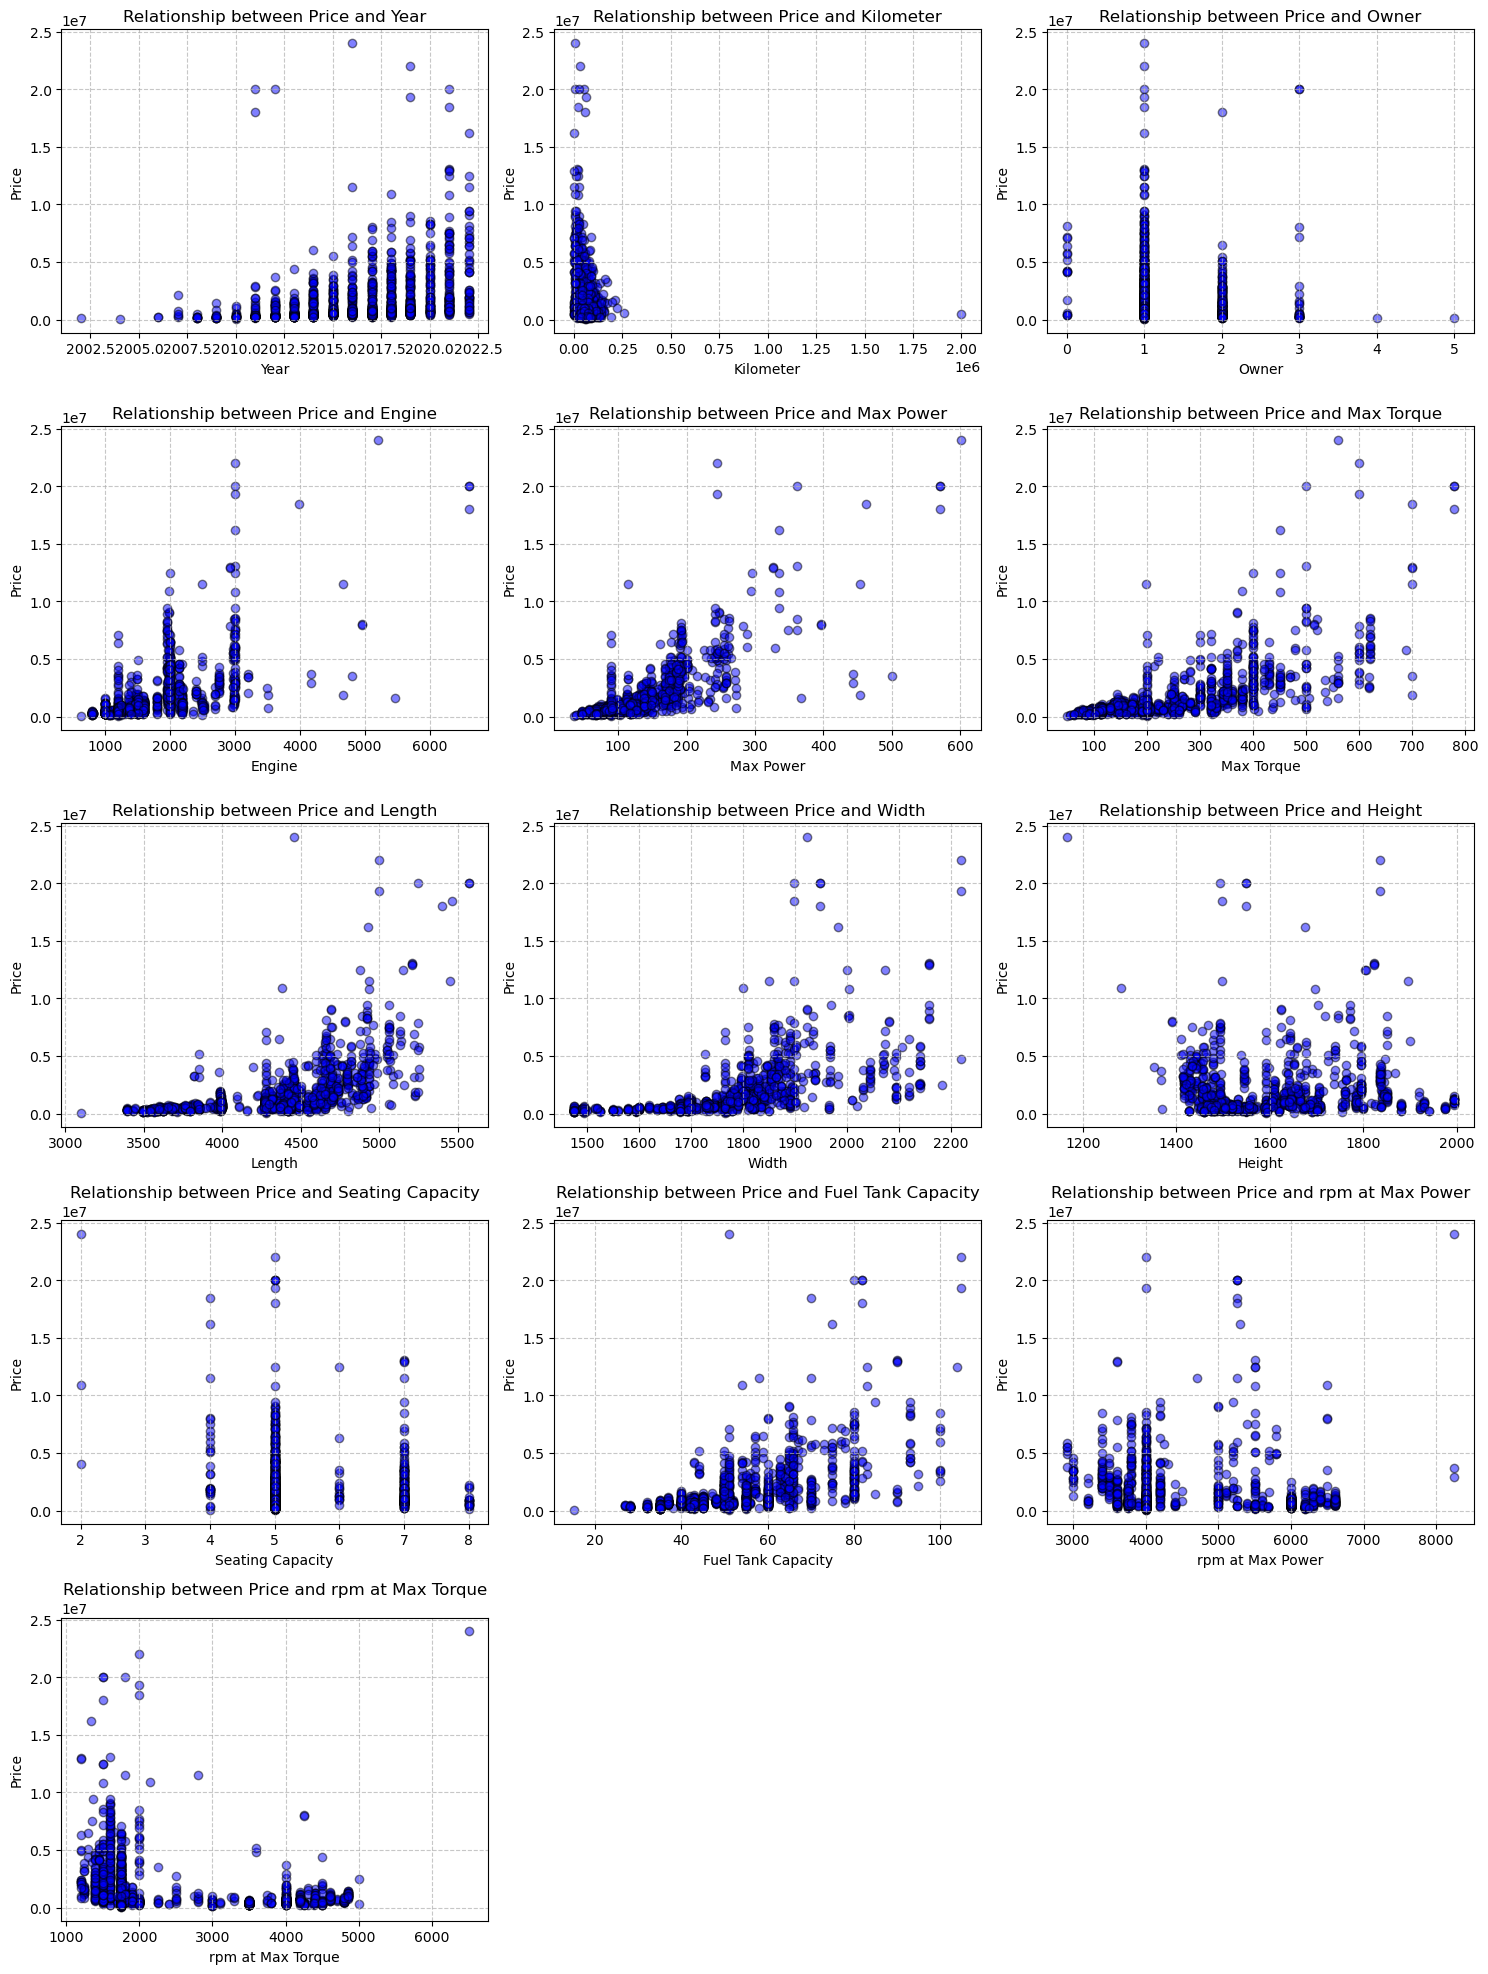
\includegraphics[width=0.9\linewidth]{img/scatter-plot.png}
    \caption{Biểu đồ phân tán so sánh giá xe theo các đặc trưng số}
    \label{fig:scatter-plot}
\end{figure}

\subsubsection{Biểu đồ hộp của các đặc trưng phi số}
\begin{figure}[H]
    \centering
    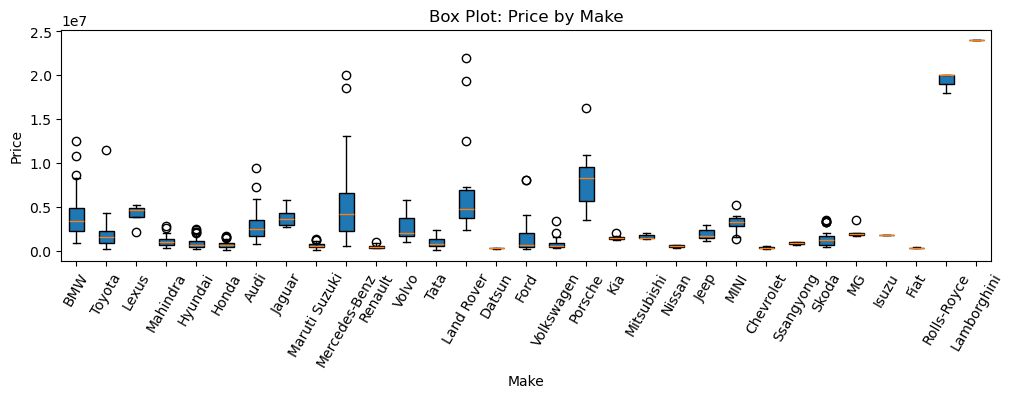
\includegraphics[width=1\linewidth]{img/boxplot-make.png}
    \caption{Biểu đồ hộp so sánh giá xe theo hãng (Make)}
    \label{fig:boxplot-make}
\end{figure}

\begin{figure}[H]
    \centering
    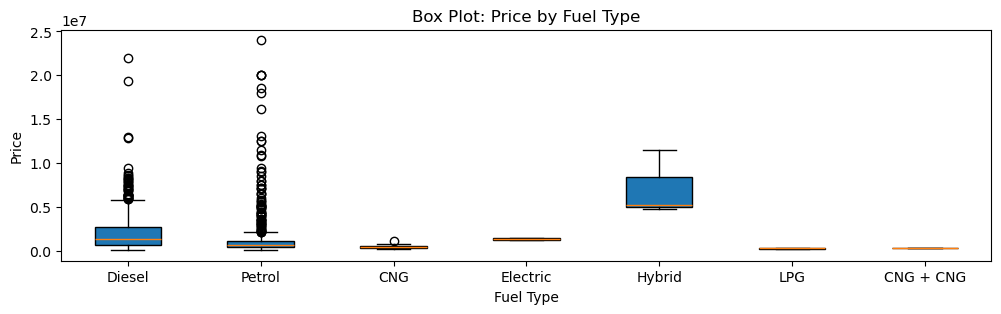
\includegraphics[width=1\linewidth]{img/boxplot-fueltype.png}
    \caption{Biểu đồ hộp so sánh giá xe theo loại nhiên liệu sử dụng (Fuel Type)}
    \label{fig:boxplot-fueltype}
\end{figure}

\begin{figure}[H]
    \centering
    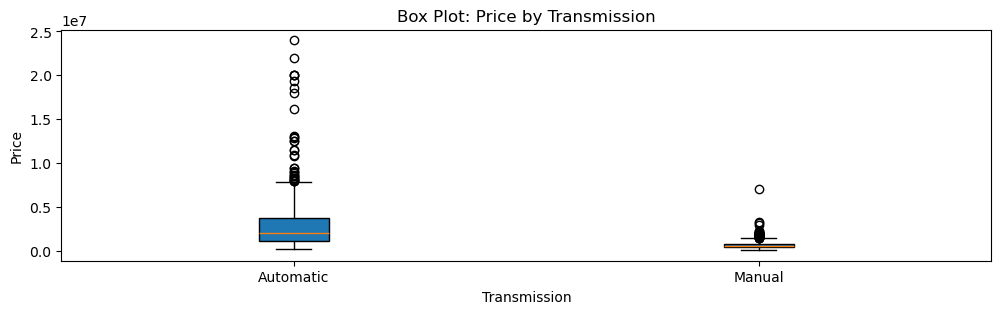
\includegraphics[width=1\linewidth]{img/boxplot-transmission.png}
    \caption{Biểu đồ hộp so sánh giá xe theo loại hộp số (Transmission)}
    \label{fig:boxplot-transmission}
\end{figure}

\begin{figure}[H]
    \centering
    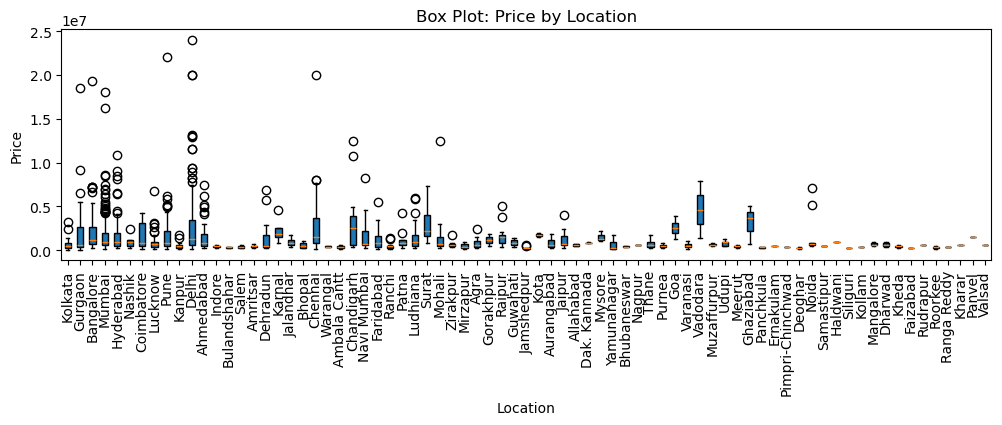
\includegraphics[width=1\linewidth]{img/boxplot-location.png}
    \caption{Biểu đồ hộp so sánh giá xe theo địa điểm (Location)}
    \label{fig:boxplot-location}
\end{figure}

\begin{figure}[H]
    \centering
    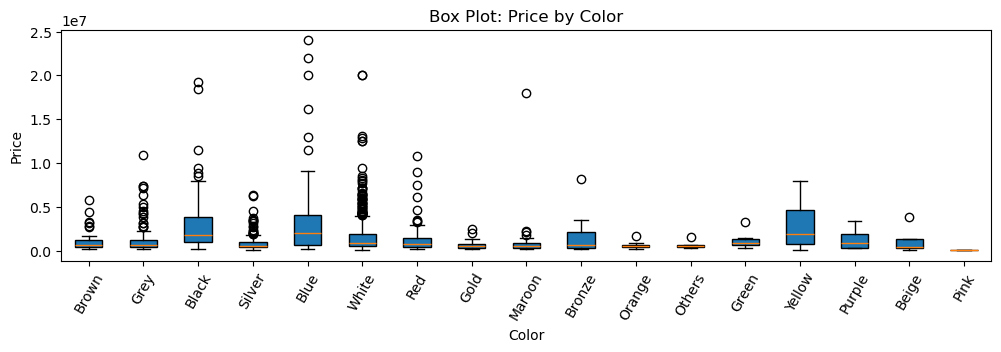
\includegraphics[width=1\linewidth]{img/boxplot-color.png}
    \caption{Biểu đồ hộp so sánh giá xe theo màu sắc (Color)}
    \label{fig:boxplot-color}
\end{figure}

\begin{figure}[H]
    \centering
    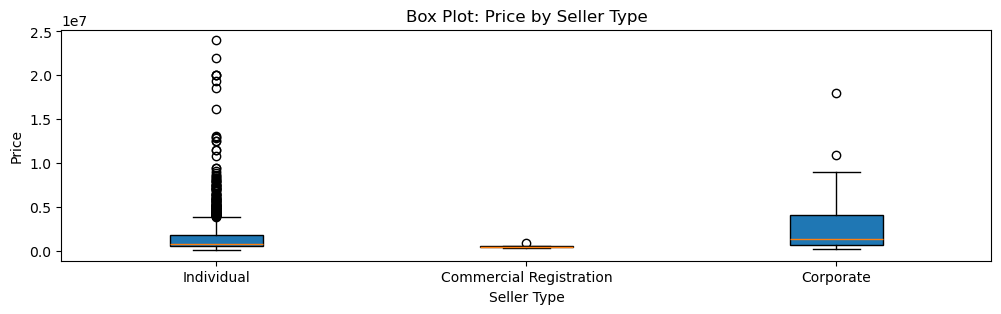
\includegraphics[width=1\linewidth]{img/boxplot-sellertype.png}
    \caption{Biểu đồ hộp so sánh giá xe theo loại người bán (Seller type)}
    \label{fig:boxplot-sellertype}
\end{figure}

\begin{figure}[H]
    \centering
    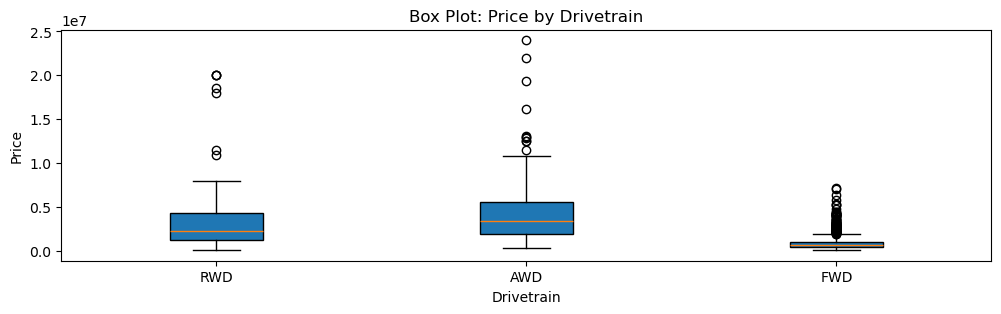
\includegraphics[width=1\linewidth]{img/boxplot-drivetrain.png}
    \caption{Biểu đồ hộp so sánh giá xe theo loại hệ dẫn động (Drivetrain)}
    \label{fig:boxplot-drivetrain}
\end{figure}

\subsubsection{Kết luận}
\paragraph{}{Từ dữ liệu được trực quan hóa, ta rút ra được một số nhận xét sau:}

\begin{itemize}
    \item Phân bố giá trị của các đặc trưng số là gần theo \textbf{phân phối chuẩn}. Ngoài ra đặc trưng giá xe (Price) và số kilomet đi được (Kilometer) lệch phải nặng (hình \ref{fig:histogram-1}). 
    \item Các đặc trưng phi số có thể được \textbf{mã hóa} thành các \textbf{đặc trưng số}.
    \item \textbf{Khoảng giá trị} của mỗi đặc trưng số là \textbf{rất khác nhau}, hoặc là rất to, hoặc là rất nhỏ. Dữ liệu cần được chuẩn hóa để giúp mô hình học tốt hơn\footnote{Xem chứng minh ở phần cơ sở toán học}.
    \item Giá xe có sự khác biệt đáng kể giữa các \textbf{hãng} và các \textbf{mẫu xe} khác nhau (hình \ref{fig:boxplot-make}), ta có thể thay thế mỗi hãng và mẫu xe bằng \textbf{giá trị trung vị} tương ứng của các xe thuộc hãng/mẫu.
    \item Giá xe Hybrid \textbf{cao hơn}\footnote{Có giá trị trung vị cao hơn và khoảng IQR đủ nhỏ} so với các loại xe sử dụng nhiên liệu khác (hình \ref{fig:boxplot-fueltype}). Tương tự, số sàn cao hơn số tự động (hình \ref{fig:boxplot-transmission}); các địa điểm bán cao hơn trung vị nhìn chung cao hơn các địa điểm còn lại (hình \ref{fig:boxplot-location}); màu đen, xanh dương và vàng cao hơn các màu khác (hình \ref{fig:boxplot-color}); công ty cao hơn cá nhân và đại lý (hình \ref{fig:boxplot-sellertype}); hệ dẫn động AWD cao hơn RWD và RWD cao hơn FWD (hình \ref{fig:boxplot-drivetrain}). Các nhận định này giúp ta \textbf{mã hóa nhị phân} (loại nhiên liệu, hộp số, địa điểm bán, màu sắc, người bán) hoặc \textbf{mã hóa theo thứ tự giá trị} (hệ dẫn động) các đặc trưng phi số, giúp mô hình học một cách hiệu quả.
\end{itemize}

\subsection{Mã hóa dữ liệu - Data encoding}
\paragraph{}{Từ những kết luận rút ra từ việc trực quan hóa dữ liệu, ta sẽ mã hóa các đặc trưng phi số về đặc trưng số. Điều này giúp tăng các đặc trưng mà mô hình có thể học.}

\begin{itemize}
    \item \textbf{Hãng xe} (Make): Thay bằng giá trung vị của các xe thuộc hãng đó.
    \item \textbf{Mẫu xe} (Model): Thay bằng giá trung vị của các xe cùng mẫu.
    \item \textbf{Loại nhiên liệu} (Fuel Type): Xe Hybrid thay bằng 1, các loại xe còn lại thay bằng 0.
    \item \textbf{Hộp số} (Transmission): Xe có hộp số tự động (Auto) thay bằng 1, hộp số sàn (Manual) thay bằng 0.
    \item \textbf{Địa điểm} (Location): Nếu giá trung vị của các xe có cùng địa điểm lớn hơn hoặc bằng giá trung vị toàn cục thì thay bằng 1; ngược lại thay bằng 0.
    \item \textbf{Màu sắc} (Color): Xe có màu trắng, xanh dương hoặc vàng thì thay bằng 1, còn lại là 0.
    \item \textbf{Loại người bán} (Seller Type): Nếu xe được bán bởi các công ty (Corporate) thì thay bằng 1, còn lại là 0.
    \item \textbf{Hệ dẫn động} (Drivetrain): FWD thay bằng 1, RWD thay bằng 2, AWD thay bằng 3.
\end{itemize}

\paragraph{}{Sau khi mã hóa các dữ liệu, ta có tổng cộng 23 đặc trưng số và không còn đặc trưng phi số.}

\subsection{Chuẩn hóa dữ liệu - Data normalization}

\paragraph{}{Từ những kết luận rút ra từ việc trực quan hóa dữ liệu, ta nhận thấy khoảng giá trị của mỗi đặc trưng số là rất khác nhau. Chẳng hạn, sức chứa chỗ ngồi (Seating capacity) nằm trong khoảng $[2, 8]$ còn công suất tối đa (Max power) nằm trong khoảng $[3000, 8000]$ (hình \ref{fig:histogram-1}). Điều đó dẫn đến một việc tất yếu là phải \textbf{chuẩn hóa dữ liệu} về một khoảng giá trị, giúp mô hình học và dự đoán tốt hơn.}

\subsubsection{Phương pháp chuẩn hóa dữ liệu}
\paragraph{}{Từ hình \ref{fig:histogram-1}, ta có nhận xét: phân phối của các đặc trưng nhìn chung tuân theo phân phối chuẩn, đặc trưng \texttt{Kilometer} có phân phối bị lệch phải. Ta sẽ áp dụng $log(x+1)$ Transformation \cite{benoit2011linear} cho \texttt{Kilometer}, sau đó áp dụng MinMax Scaler, Standard Scaler \cite{brownlee2020use} cho tất cả các đặc trưng.}
\begin{enumerate}
    \item \textbf{Log(x+1) Transformation} được sử dụng để xử lý dữ liệu bị lệch (skewed), làm cho phân phối gần với phân phối chuẩn hơn. Việc sử dụng $log(x+1)$ thay vì $log(x)$ giúp xử lý các giá trị bằng 0.

    \begin{center}
    \large $x_{scaled} = \log(x+1)$
    \end{center}

    Trong đó:
    \begin{itemize}
        \item $x_{scaled}$: Giá trị đã được chuẩn hóa.
        \item $x$: Giá trị ban đầu.
    \end{itemize}

    \item \textbf{MinMax Scaler} co giãn các giá trị về một phạm vi cụ thể, thường là từ 0 đến 1.

    \begin{center}
    \large $x_{scaled} = \frac{x - \min(x)}{\max(x) - \min(x)}$
    \end{center}

    Trong đó:
    \begin{itemize}
        \item $x_{scaled}$: Giá trị đã được chuẩn hóa.
        \item $x$: Giá trị ban đầu.
        \item $\min(x)$: Giá trị nhỏ nhất của đặc trưng trong tập dữ liệu.
        \item $\max(x)$: Giá trị lớn nhất của đặc trưng trong tập dữ liệu.
    \end{itemize}

    \item \textbf{Standard Scaler (Chuẩn hóa Z-score)} (xem \ref{label:standart scaler}) được dùng cho phương pháp PCA.
\end{enumerate}

\subsubsection{Ma trận tương quan sau mã hóa và chuẩn hóa}

\begin{figure}[H]
    \centering
    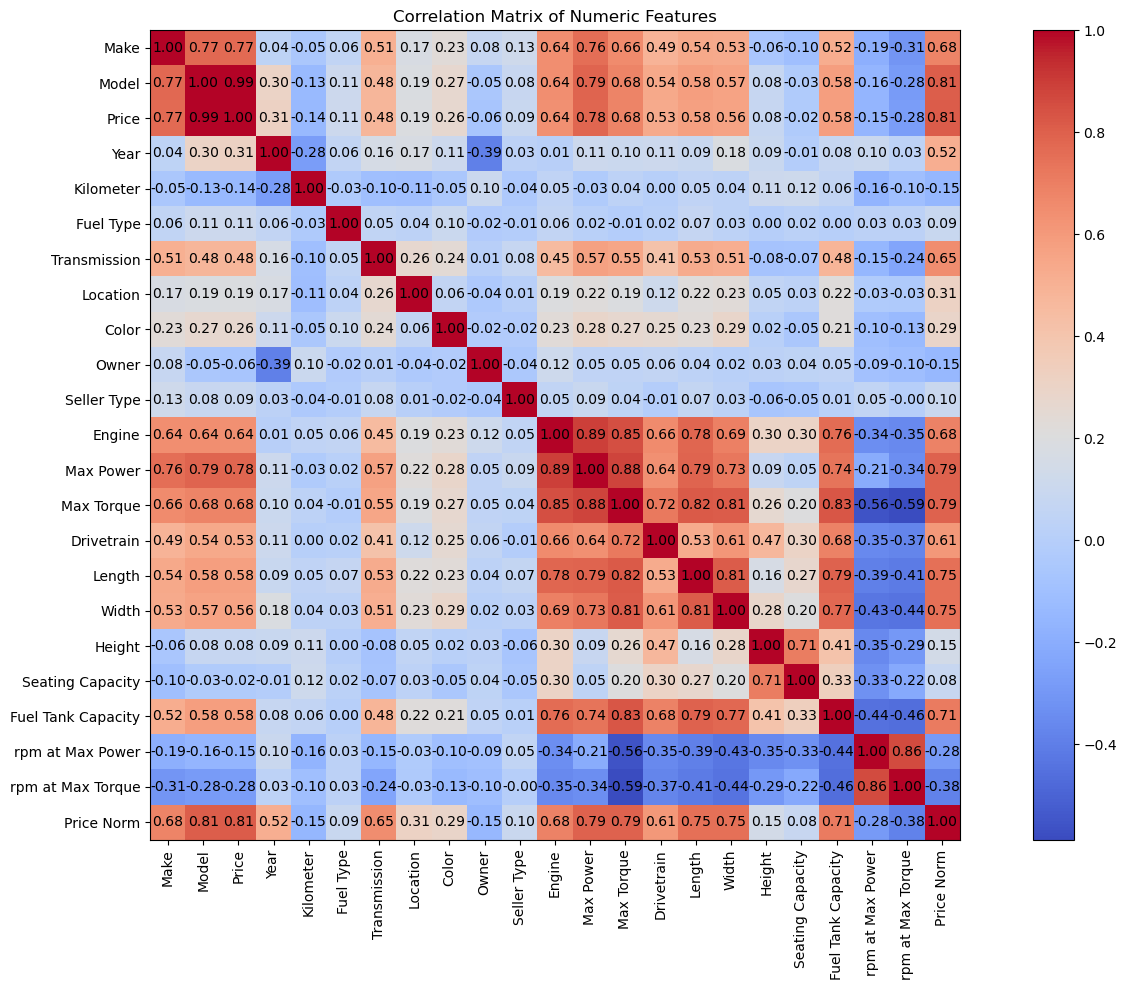
\includegraphics[width=1\linewidth]{img/corr-matrix-2.png}
    \caption{Ma trận tương quan sau khi mã hóa và chuẩn hóa dữ liệu}
    \label{fig:corr-matrix-2}
\end{figure}

\paragraph{Nhận xét:}{Sau khi mã hóa và chuẩn hóa dữ liệu, ta thấy đặc trưng \texttt{Model} có sự tương quan lớn với \texttt{Price}. Đây sẽ là cơ sở để lựa chọn đặc trưng, phục vụ các mô hình hồi quy (đặc biệt là mô hình hồi quy tuyến tính đơn).}

\pagebreak %DONE
\newpage
\section{Các phương pháp đánh giá mô hình}

\paragraph{}{Vì kết quả dự đoán của mô hình hồi quy (Regression) là giá trị liên tục, chúng ta cần các chỉ số đánh giá (evaluation metrics) \cite{regression-metrics} để định lượng "khoảng cách" hay sai số giữa \textbf{giá trị được dự đoán} (predicted) và \textbf{giá trị thực tế} (ground truth). Ba chỉ số chính dựa trên việc tính toán sai số này là MSE, RMSE, và MAE. Bên cạnh đó, chỉ số $R^2$ cũng được sử dụng rộng rãi để đánh giá mức độ phù hợp của mô hình.}

\subsection{MSE}

\paragraph{}{\textbf{MSE (Mean Squared Error)} hay \textbf{trung bình sai số bình phương} là giá trị trung bình của bình phương độ chênh lệch giữa giá trị mục tiêu và giá trị được dự đoán bởi mô hình hồi quy.}

\begin{center}
\large $MSE = \frac{1}{N}\sum_{i=1}^{N}(y_{i}-\hat{y_{i}})^2$
\end{center}

Trong đó:
\begin{itemize}
    \item $y_{i}$: Giá trị thực tế.
    \item $\hat{y_{i}}$: Giá trị được dự đoán bởi mô hình hồi quy.
    \item N: Số lượng dữ liệu.
\end{itemize}

\paragraph{Ý nghĩa:}{}
\begin{itemize}
\item MSE có miền giá trị từ $[0,+\infty ]$. 
\item Trên cùng tập dữ liệu, MSE càng nhỏ thì có độ chính xác càng cao. 
\item Vì lấy bình phương sai số nên đơn vị của MSE khác với đơn vị của kết quả dự đoán.
\item MSE nhạy cảm với các giá trị ngoại lệ (outliers) do tính bình phương. Các giá trị lớn hơn sẽ có ảnh hưởng lớn hơn đến MSE.
\end{itemize}

\subsection{RMSE}
\paragraph{}{\textbf{RMSE (Root Mean Squared Error)} hay \textbf{căn bậc hai của trung bình sai số bình phương} là giá trị căn bậc hai cho trung bình của bình phương độ chênh lệch giữa giá trị mục tiêu và giá trị được dự đoán bởi mô hình hồi quy.}

\begin{center}
\large $RMSE = \sqrt{\frac{1}{N}\sum_{i=1}^{N}(y_{i}-\hat{y_{i}})^2}$
\end{center}

Trong đó:
\begin{itemize}
    \item $y_{i}$: Giá trị thực tế.
    \item $\hat{y_{i}}$: Giá trị được dự đoán bởi mô hình hồi quy.
    \item N: Số lượng dữ liệu.
\end{itemize}

\paragraph{Ý nghĩa:}{}
\begin{itemize}
\item RMSE có miền giá trị từ $[0,+\infty ]$. 
\item Trên cùng tập dữ liệu, RMSE càng nhỏ thì có độ chính xác càng cao. 
\item Việc lấy căn bậc 2 của MSE giúp RMSE có cùng đơn vị với kết quả dự đoán, đồng thời làm giá trị RMSE không quá lớn khi số lượng điểm dữ liệu lớn.
\item RMSE cũng như MSE, nhạy cảm với các giá trị ngoại lệ (outliers) do tính bình phương.
\end{itemize}

\subsection{MAE}

\paragraph{}{\textbf{MAE (Mean Absolute Error)} hay \textbf{trung bình sai số tuyệt đối} là trung bình của giá trị tuyệt đối độ chênh lệch giữa giá trị mục tiêu và giá trị được dự đoán bởi mô hình hồi quy.}

\begin{center}
\large $MAE = \frac{1}{N}\sum_{i=1}^{N}\left| y_{i}-\hat{y_{i}} \right|$
\end{center}

Trong đó:
\begin{itemize}
    \item $y_{i}$: Giá trị thực tế.
    \item $\hat{y_{i}}$: Giá trị được dự đoán bởi mô hình hồi quy.
    \item N: Số lượng dữ liệu.
\end{itemize}

\paragraph{Ý nghĩa:}{}
\begin{itemize}
\item MAE có miền giá trị từ $[0,+\infty ]$. 
\item Trên cùng tập dữ liệu, MAE càng nhỏ thì có độ chính xác càng cao.
\item MAE không nhạy cảm với giá trị ngoại lệ (outliers) do việc sử dụng giá trị tuyệt đối.
\item MAE không phản ánh mức độ sai số cụ thể của mô hình. Nó không phân biệt được các lỗi dương và âm, chỉ cho ta biết lỗi trung bình.
\end{itemize}

\subsection{R-squared}

\paragraph{}{\textbf{Hệ số xác định} (Coefficient of Determination) \cite{xstk} là tỷ lệ của tổng sự biến thiên trong biến phụ thuộc gây ra bởi sự biến thiên của các biến độc lập (biến giải thích) so với tổng sự biến thiên toàn phần. Hệ số xác định thường được gọi là \textbf{R - bình phương} (\textbf{R-squared}), ký hiệu là $R^2$.}

\begin{center}
\large $R^{2} = \frac{SSR}{SST} = 1 - \frac{SSE}{SST} = 1 - \frac{\sum_{i=1}^{N} (y_i - \hat{y}_i)^2}{\sum_{i=1}^{N} (y_i - \bar{y})^2}$
\end{center}

Trong đó:
\begin{itemize}
    \item $y_{i}$: Giá trị thực tế.
    \item $\hat{y_{i}}$: Giá trị được dự đoán bởi mô hình hồi quy.
    \item $\bar{y}$: Giá trị trung bình của tất cả các giá trị thực tế.
    \item N: Số lượng dữ liệu.
    \item SST: Tổng bình phương toàn phần (Total Sum of Squares).
    \item SSR: Tổng bình phương hồi quy (Regression Sum of Squares).
    \item SSE: Tổng bình phương sai số (Error Sum of Squares).
\end{itemize}

\paragraph{Ý nghĩa:}{}
\begin{itemize}
\item $R^2$ có thường có miền giá trị từ $[0,1]$, nhưng có thể nhận giá trị âm\footnote{Nếu $SSE > SST$, $R^2$ sẽ âm. Điều này xảy ra khi mô hình dự đoán tệ hơn cả việc chỉ dự đoán bằng giá trị $\hat{y}$.}. Giá trị $R^2$ càng gần 1 thì mô hình càng phù hợp. 
\item $R^2$ của một mô hình hồi quy cho phép ta đánh giá mô hình tìm được có giải thích tốt cho mối liên hệ giá trị dự đoán $\hat{y}$ và giá trị thực tế $y$ hay không.
\item Với $R^2$ cao (gần 1) thì trên tổng thể, các giá trị dự đoán $\hat{y}$ có xu hướng gần với giá trị thực tế $y$.
\item $R^2$ không cho biết hiệu suất của từng dự đoán riêng lẻ. Một mô hình có $R^2$ cao vẫn có thể tạo ra một số dự đoán rất tệ cho các điểm dữ liệu cụ thể.

\end{itemize}

\pagebreak %DONE
\newpage
\section{Mô hình hồi quy tuyến tính đơn biến}
\subsection{Xây dựng mô hình}
\subsubsection{Phương pháp xây dựng}
\paragraph{}{Ta sử dụng \textbf{phương pháp bình phương tối thiểu} (Ordinary Least Squares - OLS) (xem \ref{label:simple-linear}). Phương pháp này tìm cách tối thiểu hóa tổng bình phương của các sai số giữa giá trị thực tế và giá trị dự đoán. Điều này giúp MSE của mô hình là thấp nhất.}
\subsubsection{Công thức hồi quy}
\paragraph{}{Thông qua ma trận tương quan (hình \ref{fig:corr-matrix-2}), ta thấy đặc trưng \texttt{Model} có sự tương quan lớn với \texttt{Price}. Qua thực nghiệm, \texttt{Model} là đặc trưng tốt nhất để xây dựng mô hình hồi quy tuyến tính đơn.}

\begin{center}
\large $Price = 52041.63 + 27427303.62 * Model$
\end{center}

Trong đó:
\begin{itemize}
    \item $Price$: Giá xe được dự đoán bởi mô hình
    \item $Model$: Giá trị của đặc trưng \texttt{Model} sau các quá trình xử lí dữ liệu. \footnote{Sau các quá trình tiền xử lý, mã hóa và chuẩn hóa dữ liệu. Trong đó đóng góp tích cực nhất là quá trình mã hóa đặc trưng \texttt{Model} bằng các giá trị trung vị của giá xe tương ứng.}
\end{itemize}

\subsection{Đánh giá mô hình}

\begin{figure}[H]
    \centering
    \begin{subfigure}[b]{0.48\textwidth}
        \centering
        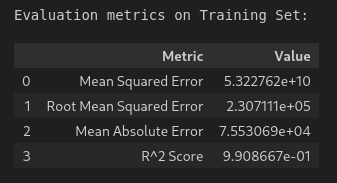
\includegraphics[width=\linewidth]{img/simple-linear-train.png}
        \caption{Đánh giá trên tập huấn luyện}
        \label{fig:simple-linear-train}
    \end{subfigure}
    \hfill
    \begin{subfigure}[b]{0.48\textwidth}
        \centering
        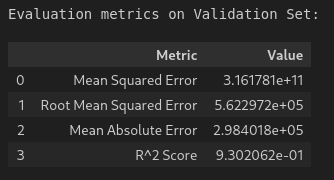
\includegraphics[width=\linewidth]{img/simple-linear-valid.png}
        \caption{Đánh giá trên tập kiểm chứng}
        \label{fig:simple-linear-valid}
    \end{subfigure}
    \caption{So sánh đánh giá mô hình trên tập huấn luyện và kiểm chứng} 
    \label{fig:simple-linear-eval}
\end{figure}

\paragraph{}{Trên tập huấn luyện, mô hình đạt MSE là $5.322762 * 10^{10}$ và R² là $0.9908$, cho thấy mô hình rất khớp với dữ liệu đã thấy. Tuy nhiên, trên tập kiểm chứng, MSE tăng lên đáng kể thành $3.161781 * 10^{11}$ và R² giảm xuống còn 0.9302.}

\paragraph{}{Mặc dù R² trên tập kiểm chứng vẫn khá cao, sự gia tăng đáng kể của các chỉ số lỗi (MSE tăng gấp 6 lần) cho thấy dấu hiệu của hiện tượng overfitting. Mô hình đã học thuộc một số đặc điểm nhiễu của tập huấn luyện và khả năng tổng quát hóa trên dữ liệu mới bị hạn chế hơn. Điều này cũng có thể quan sát thấy trong hình \ref{fig:simple-linear}, nơi các điểm dữ liệu kiểm chứng phân tán rộng hơn quanh đường dự đoán so với tập huấn luyện. Tuy nhiên, điều này có thể  chấp nhận được vì đây chỉ là mô hình hồi quy tuyến tính đơn.}

\begin{figure}[H]
    \centering
    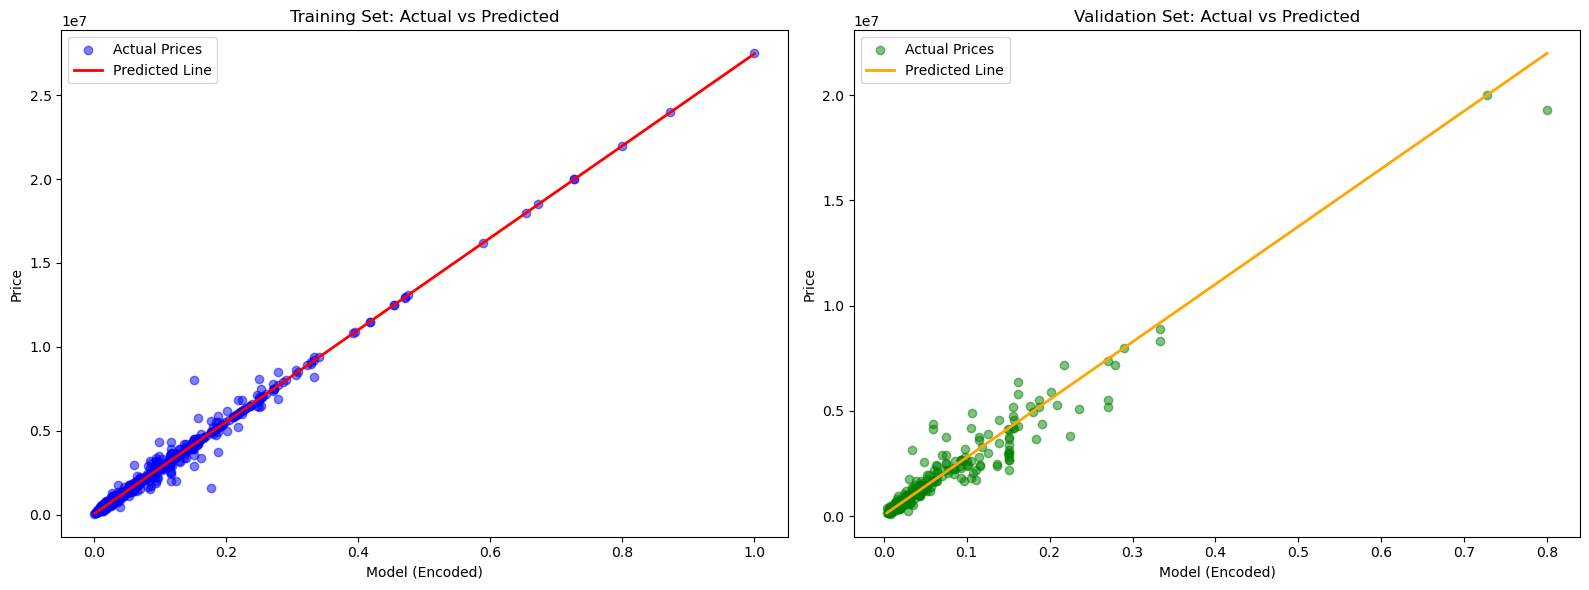
\includegraphics[width=1\linewidth]{img/simple-linear.png}
    \caption{Đường thẳng hồi quy dự đoán so với thực tế, trên tập huấn luyện và kiểm chứng}
    \label{fig:simple-linear}
\end{figure}

\pagebreak %DONE
\newpage
\section{Mô hình hồi quy tuyến tính đa biến}

\subsection{Giới thiệu}

\subsubsection{Khái niệm hồi quy tuyến tính đa biến}

Hồi quy tuyến tính đa biến \cite{geeksforgeeks-ml} (Multiple Linear Regression - MLR) là một phương pháp thống kê mở rộng từ hồi quy tuyến tính đơn giản, được sử dụng để mô hình hóa mối quan hệ giữa một biến phụ thuộc và nhiều biến độc lập. Mô hình có dạng tổng quát như sau:

\[
y = b + \theta_1 x_1 + \theta_2 x_2 + \cdots + \theta_p x_p
\]

Trong đó:
\begin{itemize}
    \item $y$ là biến phụ thuộc (biến kết quả)
    \item $x_1, x_2, \ldots, x_p$ là các biến độc lập (biến dự đoán)
    \item $b$ là hệ số chặn (intercept)
    \item $\theta_1, \theta_2, \ldots, \theta_p$ là các hệ số hồi quy
\end{itemize}

Mục tiêu của thuật toán là tìm ra siêu phẳng phù hợp nhất có thể dự đoán các giá trị dựa trên các biến độc lập. Mô hình hồi quy học một hàm từ tập dữ liệu (với các giá trị $X$ và $Y$ đã biết) và sử dụng nó để dự đoán giá trị $Y$ từ các giá trị $X$ mới.

\subsubsection{So sánh với hồi quy tuyến tính đơn giản}

Hồi quy tuyến tính đa biến khác biệt với hồi quy tuyến tính đơn giản ở những điểm chính sau:

\begin{table}[H]
\centering
\begin{tabular}{|p{5cm}|p{5cm}|p{5cm}|}
\hline
\textbf{Đặc điểm} & \textbf{Hồi quy đơn giản} & \textbf{Hồi quy đa biến} \\
\hline
Số biến độc lập & Một biến & Nhiều biến \\
\hline
Mô hình toán học & $Y = b + \theta_1 X$ & $Y = b + \theta_1 x_1 + \dots + \theta_p x_p$ \\
\hline
Diễn giải hình học & Đường thẳng trong không gian 2 chiều & Siêu phẳng trong không gian $p+1$ chiều \\
\hline
\end{tabular}
\caption{So sánh giữa hồi quy tuyến tính đơn giản và đa biến}
\label{tab:comparison}
\end{table}

Hồi quy tuyến tính đa biến vượt trội hơn so với hồi quy tuyến tính đơn giản trong việc:

\begin{itemize}
    \item Cung cấp khả năng phân tích đa chiều do có thể tận dụng toàn bộ đặc điểm từ dữ liệu
    \item Tăng khả năng dự báo chính xác khi có nhiều yếu tố ảnh hưởng
\end{itemize}

\subsection{Xây dựng mô hình}
\subsubsection{Ma trận hóa}

Mô hình hồi quy tuyến tính đa biến đã được giới thiệu với dạng tổng quát như sau:

\begin{equation}
    y = b + \theta_1 x_1 + \theta_2 x_2 + \cdots + \theta_p x_p
\end{equation}

Trong quá trình phân tích với bộ dữ liệu lớn, xử lý tuần tự từng mẫu trở nên kém hiệu quả. Cụ thể, với tập dữ liệu bao gồm 1647 mẫu quan sát, việc áp dụng phương pháp ma trận hóa không chỉ tối ưu hóa khả năng tính toán song song mà còn cung cấp một cách biểu diễn toán học chặt chẽ và súc tích. 

Đối với một quan sát đơn lẻ với $p$ đặc trưng (features), ta có thể biểu diễn giá trị dự đoán thông qua nhân ma trận như sau:

\[
    y = 
    \begin{bmatrix}
        x_{1} & x_{2} & \dots & x_{p} \\
    \end{bmatrix}
    _{\text{$1 \times p$}}
    \begin{bmatrix}
        \theta_{1} \\
        \theta_{2} \\
        \vdots \\
        \theta_{p}
    \end{bmatrix}
    _{\text{$p \times 1$}}
    +
    b
\]

Khi mở rộng phương pháp này cho toàn bộ tập dữ liệu với $n$ quan sát, ta thu được biểu diễn ma trận tổng quát của mô hình hồi quy:

\[
    \begin{bmatrix}
        y_1 \\
        y_2 \\
        \vdots \\
        y_n
    \end{bmatrix}
    _{\text{$n \times 1$}}
    = 
    \begin{bmatrix}
        x_{11} & x_{12} & \dots & x_{1p} \\
        x_{21} & x_{22} & \dots & x_{2p} \\
        \vdots & \vdots & \ddots & \vdots \\
        x_{n1} & x_{n2} & \dots & x_{np} \\
    \end{bmatrix}
    _{\text{$n \times p$}}
    \begin{bmatrix}
        \theta_{1} \\
        \theta_{2} \\
        \vdots \\
        \theta_{p}
    \end{bmatrix}
    _{\text{$p \times 1$}}
    +
    \begin{bmatrix}
        b_{1} \\
        b_{2} \\
        \vdots \\
        b_{n}
    \end{bmatrix}
    _{\text{$n \times 1$}}
\]

Phương trình này có thể được biểu diễn một cách súc tích hơn trong ký hiệu ma trận:

\begin{equation}
    \label{eq:mlr}
    \mathbf{Y} = \mathbf{X}\boldsymbol{\theta} + \mathbf{b}
\end{equation}

Trong đó:
\begin{itemize}
    \item $\mathbf{Y} \in \mathbb{R}^{n \times 1}$ là vector cột chứa $n$ giá trị phụ thuộc
    \item $\mathbf{X} \in \mathbb{R}^{n \times p}$ là ma trận chứa $n$ mẫu quan sát với $p$ đặc trưng cho mỗi mẫu
    \item $\boldsymbol{\theta} \in \mathbb{R}^{p \times 1}$ là vector tham số cần ước lượng
    \item $\mathbf{b} \in \mathbb{R}^{n \times 1}$ là vector hệ số chặn (intercept) với mỗi phần tử đều bằng nhau và bằng b
\end{itemize}

\subsubsection{Hàm mất mát}

Trong quá trình xây dựng mô hình hồi quy tuyến tính đa biến, việc lựa chọn hàm mất mát (loss function) đóng vai trò quyết định đến hiệu suất và khả năng hội tụ của mô hình. Sau khi cân nhắc các phương pháp khác nhau, Mean Squared Error (MSE) 4.1 được quyết định làm hàm mất mát chính:

Biểu diễn dưới dạng ma trận, hàm mất mát MSE có thể được viết như sau:

\[
   \mathcal{L}(\boldsymbol{\theta}, \boldsymbol{b}) = \frac{1}{n} \|\mathbf{Y} - \mathbf{X}\boldsymbol{\theta} - \mathbf{b}\|_2^2
\]

\subsubsection{Gradient Descent}

Mô hình này sẽ áp dụng Gradient Descent, là một thuật toán tối ưu hóa cơ bản nhất và quan trọng nhất trong lĩnh vực học máy, đã được đề cập ở 2.2. 

\paragraph{Vai trò quan trọng của tốc độ học $\alpha$} Việc lựa chọn tốc độ học $\alpha$ cho thuật toán Gradient Descent có ảnh hưởng quyết định đến hiệu quả của quá trình huấn luyện:

\begin{itemize}
    \item Nếu $\alpha$ có giá trị phù hợp: Mô hình sẽ hội tụ đến điểm cực tiểu của hàm mất mát sau một số lần cập nhật.
    
    \item Nếu $\alpha$ quá lớn: Mô hình sẽ liên tục \textbf{overshoot} (vượt lố) điểm cực tiểu, dao động qua lại giữa các điểm có giá trị mất mát lớn hơn. Sai số tích lũy sau mỗi lần cập nhật có thể dẫn đến hiện tượng phân kỳ, trong đó hàm mất mát có xu hướng tăng thay vì giảm.
    
    \item Nếu $\alpha$ quá nhỏ: Quá trình hội tụ sẽ diễn ra rất chậm, đòi hỏi số lượng vòng lặp lớn và tăng thời gian huấn luyện.
\end{itemize}

\begin{figure}[H]
    \centering
    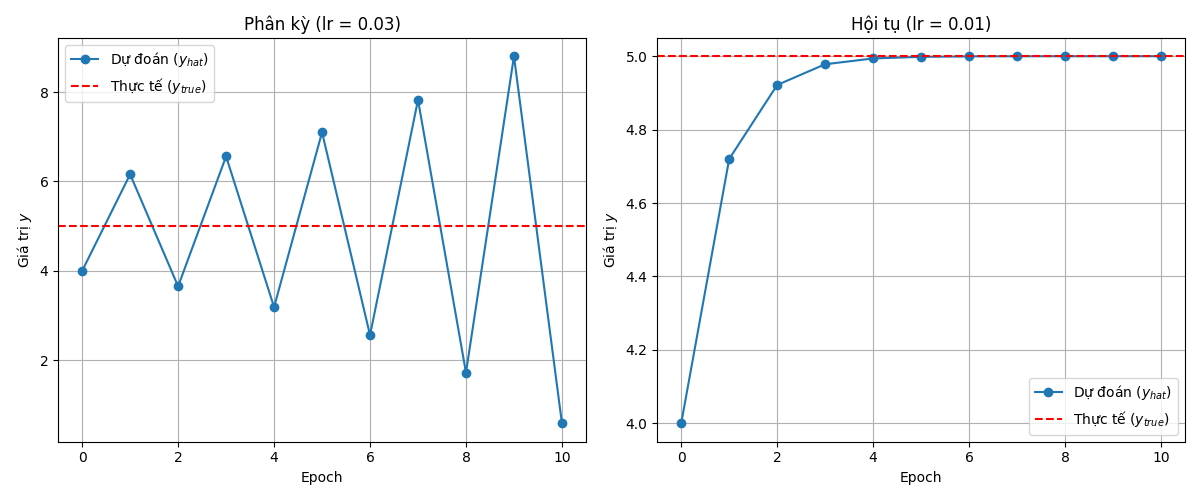
\includegraphics[width=1\linewidth]{img_multiple/diverge_converge.png}
    \caption{Hiện tượng phân kỳ và hội tụ tùy thuộc vào cách chọn tốc độ học}
    \label{fig:diverge_converge}
\end{figure}

\subsection{Quá trình huấn luyện}
\paragraph{Biểu diễn ma trận của mô hình}
Trong mô hình hồi quy tuyến tính đa biến với \( n \) mẫu và \( p \) biến độc lập, ta có thể biểu diễn mô hình dưới dạng ma trận mở rộng để gộp cả tham số bias \( b \) vào:

\begin{itemize}
    \item \( \tilde{X} \in \mathbb{R}^{n \times (p+1)} \): Ma trận dữ liệu mở rộng, với cột đầu tiên là toàn số 1:
    \[
        \tilde{X} = 
        \begin{bmatrix}
            1 & x_{11} & x_{12} & \cdots & x_{1p} \\
            1 & x_{21} & x_{22} & \cdots & x_{2p} \\
            \vdots & \vdots & \vdots & \ddots & \vdots \\
            1 & x_{n1} & x_{n2} & \cdots & x_{np}
        \end{bmatrix}
    \]
    
    \item \( \tilde{\theta} \in \mathbb{R}^{(p+1) \times 1} \): Vector tham số mở rộng, bao gồm cả bias như phần tử đầu tiên:
    \[
        \tilde{\theta} = 
        \begin{bmatrix}
            b \\
            \theta_1 \\
            \theta_2 \\
            \vdots \\
            \theta_p
        \end{bmatrix}
    \]
\end{itemize}

Với cách biểu diễn mở rộng này, mô hình dự đoán có dạng:

\[
    \hat{Y} = \tilde{X}\tilde{\theta}
\]

Trong đó mỗi phần tử \(\hat{y}_i\) của vector \(\hat{Y}\) được tính như sau:

\[
    \hat{y}_i = b + \sum_{j=1}^{p} \theta_j x_{ij}
\]

\paragraph{Đạo hàm ma trận của hàm mất mát}
Hàm mất mát Mean Squared Error (MSE) với cách biểu diễn mở rộng có dạng:

\[
    \mathcal{L}(\tilde{\theta}) = \frac{1}{n} (Y - \tilde{X}\tilde{\theta})^T (Y - \tilde{X}\tilde{\theta})
\]

Gradient của hàm mất mát theo vector tham số mở rộng \(\tilde{\theta}\) là:

\[
    \frac{\partial \mathcal{L}}{\partial \tilde{\theta}} = -\frac{2}{n} \tilde{X}^T(Y - \hat{Y})
\]

Khi phân tích thành các thành phần:

\[
    \frac{\partial \mathcal{L}}{\partial \tilde{\theta}} = -\frac{2}{n} 
    \begin{bmatrix}
        \sum_{i=1}^n (y_i - \hat{y}_i) \\
        \sum_{i=1}^n (y_i - \hat{y}_i)x_{i1} \\
        \sum_{i=1}^n (y_i - \hat{y}_i)x_{i2} \\
        \vdots \\
        \sum_{i=1}^n (y_i - \hat{y}_i)x_{ip}
    \end{bmatrix}
\]

\paragraph{Cập nhật tham số thông qua ma trận}
Sử dụng thuật toán Gradient Descent, ta cập nhật vector tham số mở rộng \(\tilde{\theta}\) như sau:

\[
    \tilde{\theta}^{(t+1)} = \tilde{\theta}^{(t)} + \frac{2\alpha}{n} \tilde{X}^T(Y - \hat{Y}^{(t)})
\]

Cụ thể:

\[
\begin{bmatrix}
    b^{(t+1)} \\
    \theta_1^{(t+1)} \\
    \theta_2^{(t+1)} \\
    \vdots \\
    \theta_p^{(t+1)}
\end{bmatrix} = 
\begin{bmatrix}
    b^{(t)} \\
    \theta_1^{(t)} \\
    \theta_2^{(t)} \\
    \vdots \\
    \theta_p^{(t)}
\end{bmatrix} + 
\frac{2\alpha}{n} 
\begin{bmatrix}
    \sum_{i=1}^n (y_i - \hat{y}_i^{(t)}) \\
    \sum_{i=1}^n (y_i - \hat{y}_i^{(t)})x_{i1} \\
    \sum_{i=1}^n (y_i - \hat{y}_i^{(t)})x_{i2} \\
    \vdots \\
    \sum_{i=1}^n (y_i - \hat{y}_i^{(t)})x_{ip}
\end{bmatrix}
\]

Với \(\alpha\) là tốc độ học và \(t\) là chỉ số của bước lặp trong quá trình huấn luyện.

\subsection{Thử nghiệm mô hình}
Để đảm bảo hiệu năng tối ưu, ta tiến hành thử nghiệm mô hình thông qua nhiều phương pháp huấn luyện khác nhau nhằm xác định cấu hình nào mang lại kết quả tốt nhất.

\subsubsection{Kiến trúc mô hình}
\paragraph{Mô hình cơ sở (base model)}Mô hình cơ sở chính là mô hình tuyến tính đa biến chuẩn mà ta đã thảo luận ở \eqref{eq:mlr}.

\begin{figure}[H]
    \centering
    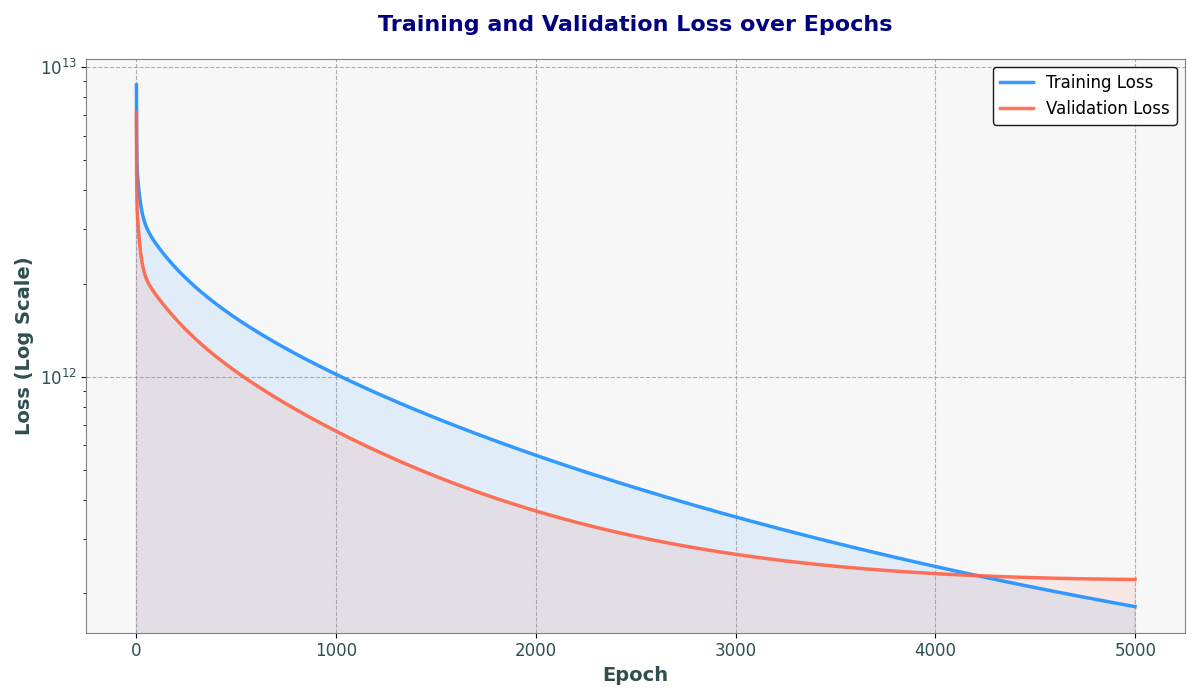
\includegraphics[width=0.9\textwidth]{img_multiple/loss_base.png} % Hình lớn chiếm 90% chiều rộng
    \caption{Giá trị hàm mất mát qua từng epoch (base model)}
    \label{fig:loss_base}
\end{figure}

% Figure 2: Hai subfigure nằm ngang bên dưới
\begin{figure}[H]
    \centering
    \begin{subfigure}[b]{0.48\textwidth}
        \centering
        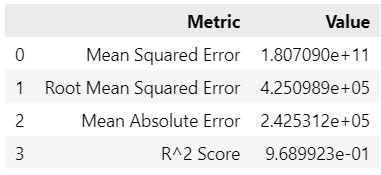
\includegraphics[width=\linewidth]{img_multiple/metrics_base_train.png}
        \caption{Đánh giá trên tập huấn luyện}
    \end{subfigure}
    \hfill
    \begin{subfigure}[b]{0.48\textwidth}
        \centering
        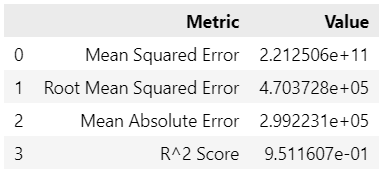
\includegraphics[width=\linewidth]{img_multiple/metrics_base_val.png}
        \caption{Đánh giá trên tập kiểm chứng}
    \end{subfigure}
    \caption{So sánh đánh giá mô hình trên tập huấn luyện và kiểm chứng (base model)} 
\end{figure}

\textit{Nhận xét:} Mô hình cơ sở chưa thông qua các phương pháp gì đặc biệt nhưng vẫn đạt kết quả khá tốt. 

\paragraph{Mô hình không thành phần bias}Theo lý thuyết, việc loại bỏ thành phần bias thường không được khuyến khích vì nó làm giảm đáng kể khả năng biểu diễn và độ phức tạp của mô hình. Để minh họa rõ hơn vấn đề này, ta xét một trường hợp đơn giản với mô hình hồi quy một biến:

\begin{figure}[H]
    \centering
    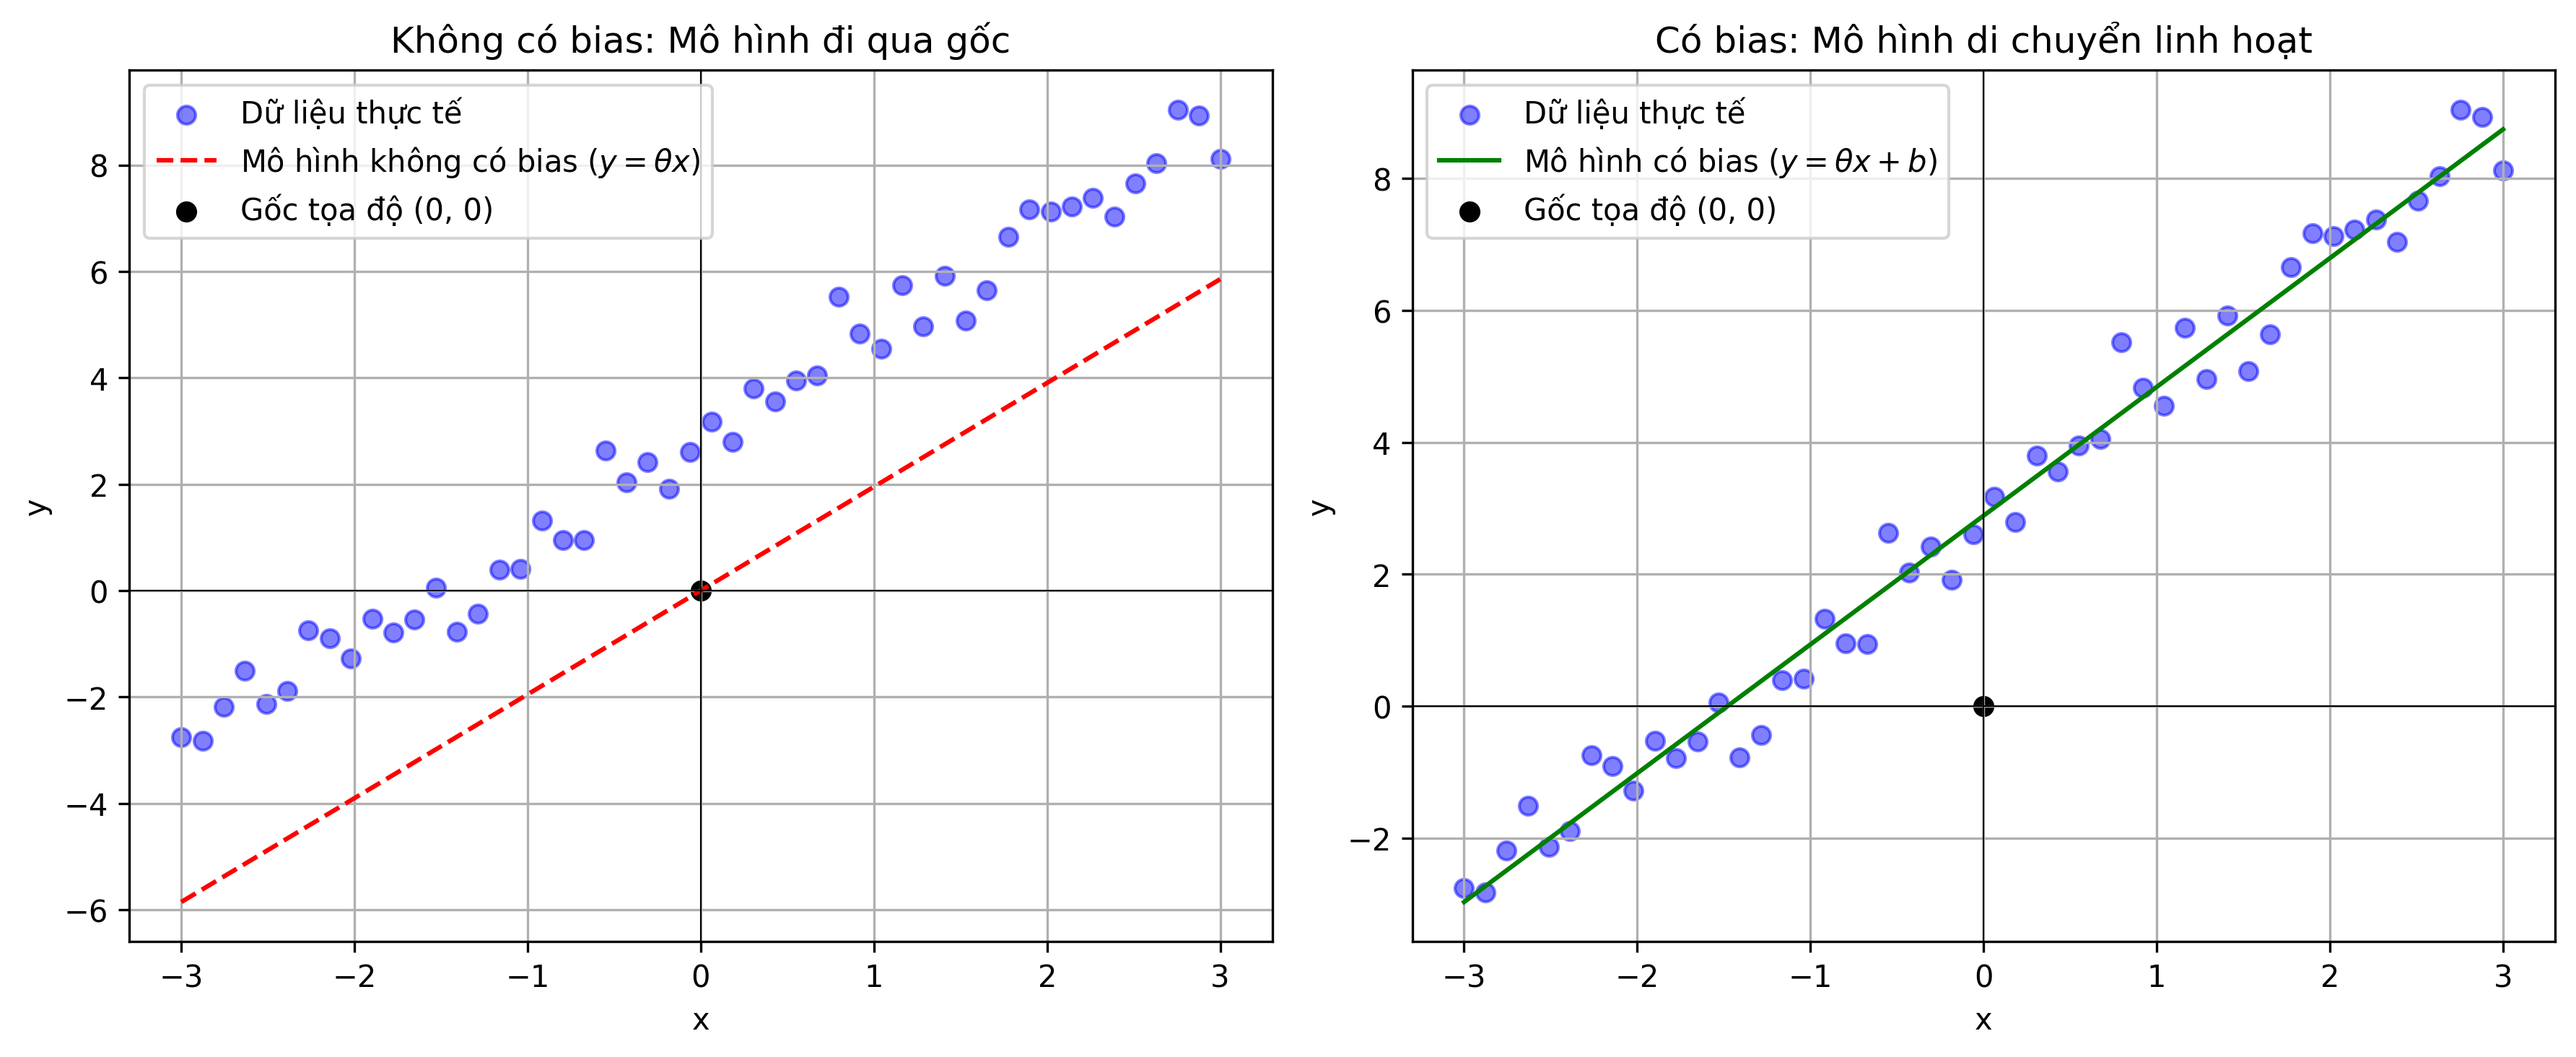
\includegraphics[width=1\linewidth]{img_multiple/bias_comparison_separate.png}
    \caption{So sánh hiệu năng giữa mô hình có và không có thành phần bias}
    \label{fig:bias_comparison}
\end{figure}

Ở mô hình không có bias, mặc dù mô hình học được xu hướng của dữ liệu nhưng do bị giới hạn ở gốc tọa độ, nó không thể nắm bắt được chính xác các mối quan hệ của chúng.

\begin{figure}[H]
    \centering
    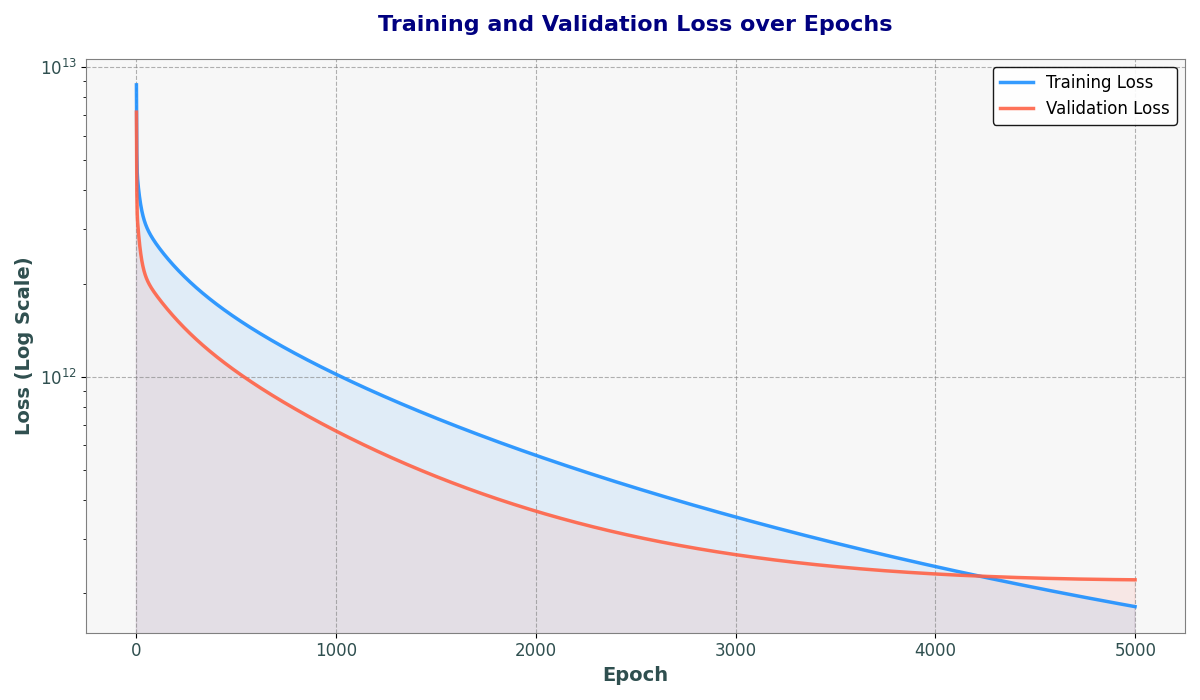
\includegraphics[width=0.9\textwidth]{img_multiple/loss_no_bias.png} % Hình lớn chiếm 90% chiều rộng
    \caption{Giá trị hàm mất mát qua từng epoch (no bias)}
    \label{fig:loss_no_bias}
\end{figure}

% Figure 2: Hai subfigure nằm ngang bên dưới
\begin{figure}[H]
    \centering
    \begin{subfigure}[b]{0.48\textwidth}
        \centering
        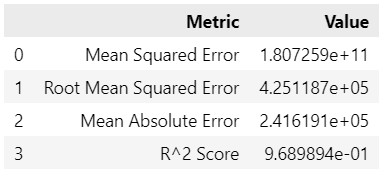
\includegraphics[width=\linewidth]{img_multiple/metrics_no_bias_train.png}
        \caption{Đánh giá trên tập huấn luyện}
    \end{subfigure}
    \hfill
    \begin{subfigure}[b]{0.48\textwidth}
        \centering
        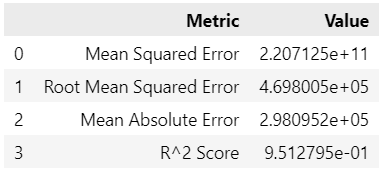
\includegraphics[width=\linewidth]{img_multiple/metrics_no_bias_val.png}
        \caption{Đánh giá trên tập kiểm chứng}
    \end{subfigure}
    \caption{So sánh đánh giá mô hình trên tập huấn luyện và kiểm chứng (no bias)} 
\end{figure}

\subsubsection{Chuyển hóa biến mục tiêu}
Trong các thử nghiệm trước, ta đã sử dụng các đặc trưng đã chuẩn hóa để dự đoán giá nhà ở giá trị gốc. Phần này trình bày các phương pháp chuyển hóa biến mục tiêu nhằm đưa giá trị về phạm vi nhỏ hơn, tạo điều kiện thuận lợi cho quá trình huấn luyện và cải thiện hiệu suất của mô hình.

\paragraph{Phương pháp Min-Max Scaling}
Phép biến đổi Min-Max Scaling được áp dụng theo công thức sau:
\[
    y_{\text{transformed}} = \frac{y_{\text{original}} - y_{\text{min}}}{y_{\text{max}} - y_{\text{min}}}
\]

Phương pháp này chuẩn hóa dữ liệu về khoảng [0, 1], giữ nguyên hình dạng phân phối gốc nhưng thu hẹp phạm vi giá trị.

\begin{figure}[H]
    \centering
    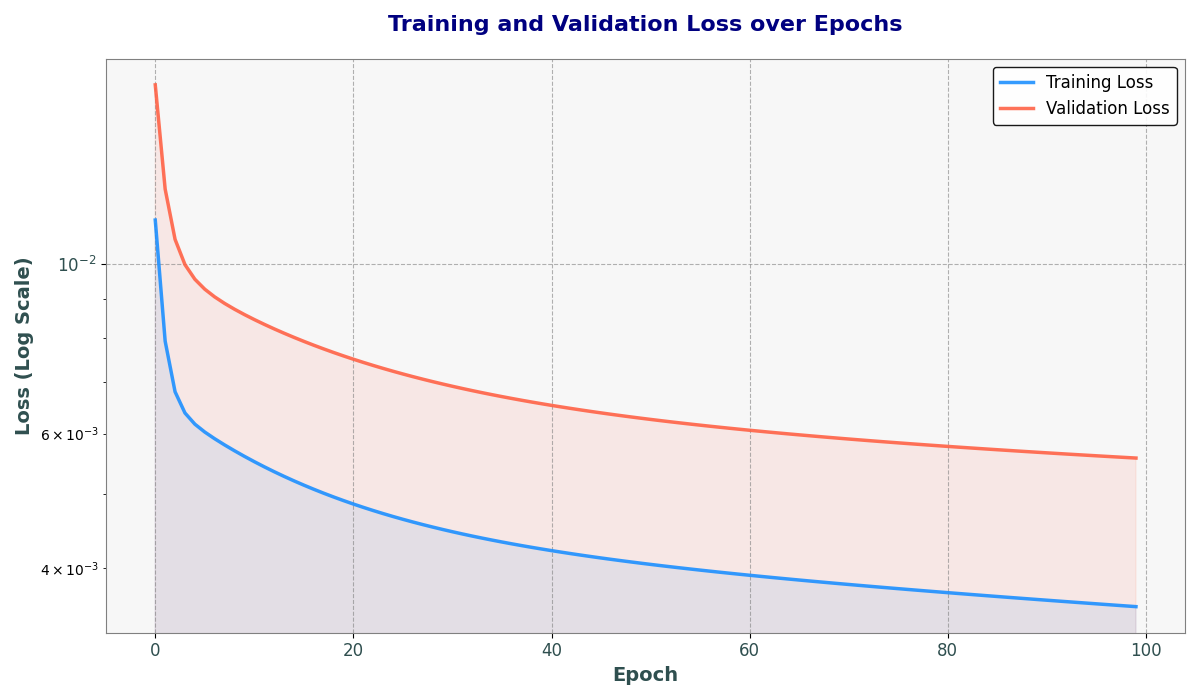
\includegraphics[width=0.9\textwidth]{img_multiple/loss_min_max.png} % Hình lớn chiếm 90% chiều rộng
    \caption{Giá trị hàm mất mát qua từng epoch (Min-Max Scaling)}
    \label{fig:loss_min_max}
\end{figure}

% Figure 2: Hai subfigure nằm ngang bên dưới
\begin{figure}[H]
    \centering
    \begin{subfigure}[b]{0.48\textwidth}
        \centering
        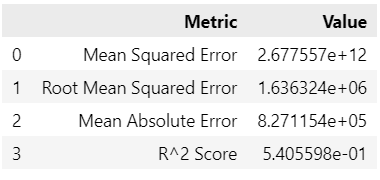
\includegraphics[width=\linewidth]{img_multiple/metrics_min_max_train.png}
        \caption{Đánh giá trên tập huấn luyện}
    \end{subfigure}
    \hfill
    \begin{subfigure}[b]{0.48\textwidth}
        \centering
        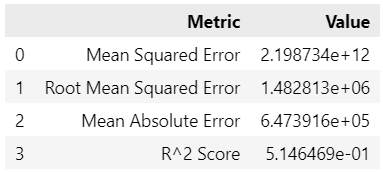
\includegraphics[width=\linewidth]{img_multiple/metrics_min_max_val.png}
        \caption{Đánh giá trên tập kiểm chứng}
    \end{subfigure}
    \caption{So sánh đánh giá mô hình trên tập huấn luyện và kiểm chứng (Min-Max Scaling)} 
\end{figure}

\textit{Nhận xét:} Sau khi chuyển hóa, tốc độ hội tụ của mô hình tăng nhanh đáng kể (chỉ sau khoảng 10 epoch). Hàm mất mát giảm mạnh ở một vài epoch đầu và sườn dốc bắt đầu thoải hơn (giảm chậm) ở các epoch sau chứng tỏ mô hình đã hội tụ.

\paragraph{}{\textbf{Phương pháp chuẩn hóa (Standardization)} \cite{kaggle-standardization}, \cite{youtube-standardization-normalization}: }
Phương pháp chuẩn hóa áp dụng công thức:
\[
    y_{\text{transformed}} = \frac{y_{\text{original}} - \mu_{y}}{\sigma_{y}}
\]

Trong đó $\mu_{y}$ là giá trị trung bình và $\sigma_{y}$ là độ lệch chuẩn của biến mục tiêu. Phương pháp này chuyển đổi dữ liệu về phân phối có trung bình bằng 0 và phương sai bằng 1.

\begin{figure}[H]
    \centering
    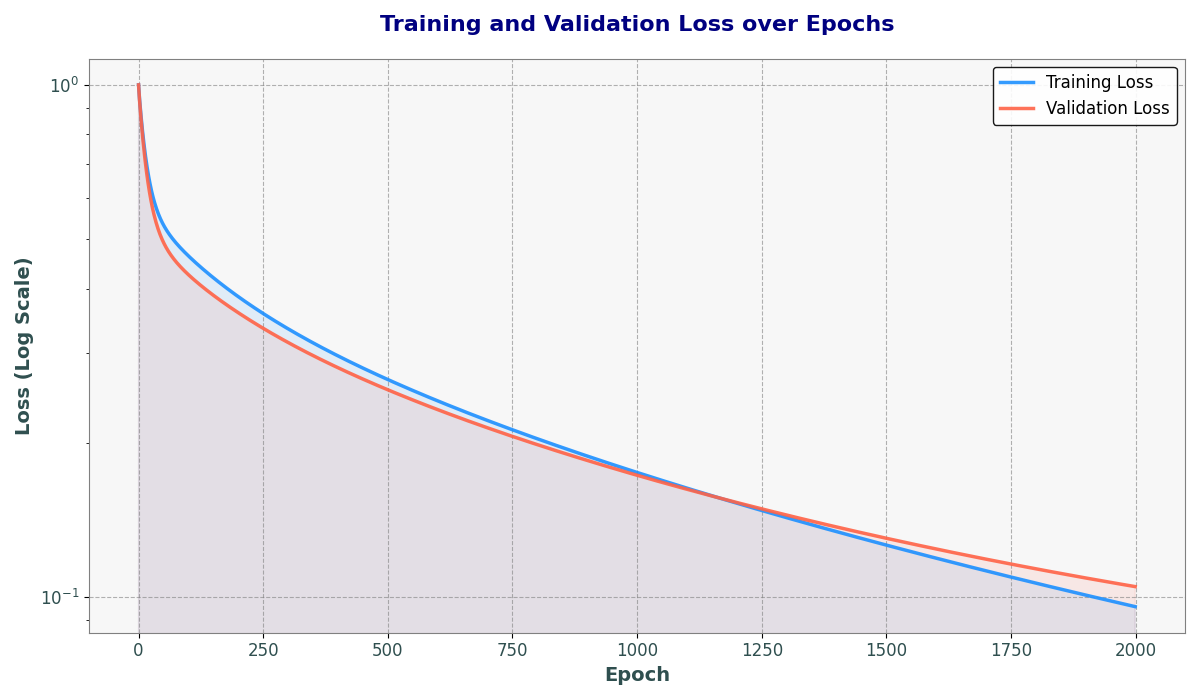
\includegraphics[width=0.9\textwidth]{img_multiple/loss_standardization.png} % Hình lớn chiếm 90% chiều rộng
    \caption{Giá trị hàm mất mát qua từng epoch (Standardization)}
    \label{fig:loss_standardization}
\end{figure}

% Figure 2: Hai subfigure nằm ngang bên dưới
\begin{figure}[H]
    \centering
    \begin{subfigure}[b]{0.48\textwidth}
        \centering
        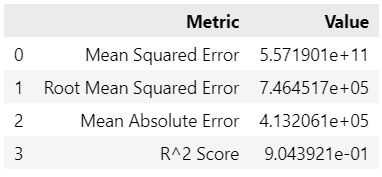
\includegraphics[width=\linewidth]{img_multiple/metrics_standard_train.png}
        \caption{Đánh giá trên tập huấn luyện}
    \end{subfigure}
    \hfill
    \begin{subfigure}[b]{0.48\textwidth}
        \centering
        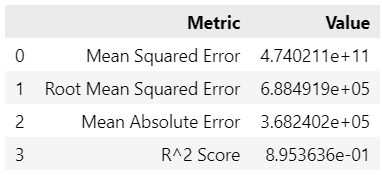
\includegraphics[width=\linewidth]{img_multiple/metrics_standard_val.png}
        \caption{Đánh giá trên tập kiểm chứng}
    \end{subfigure}
    \caption{So sánh đánh giá mô hình trên tập huấn luyện và kiểm chứng (Standardization)} 
\end{figure}

\subsubsection{Regularization}
\paragraph{}{Regularization là phương pháp kiểm soát độ phức tạp của mô hình thông qua việc thêm các ràng buộc vào hàm mục tiêu trong quá trình tối ưu hóa. Phương pháp này đóng vai trò quan trọng trong việc giảm thiểu hiện tượng \textit{quá khớp} (overfitting) trên tập huấn luyện, đồng thời tăng cường khả năng \textit{tổng quát hóa} (generalization) của mô hình. Kết quả là mô hình có thể duy trì độ chính xác cao khi dự đoán trên dữ liệu mới chưa từng được tiếp xúc trong quá trình huấn luyện.}

\paragraph{Hồi quy Lasso (Lasso Regression)}
Phương pháp hồi quy Lasso áp dụng kỹ thuật điều chuẩn L1 thông qua việc bổ sung thành phần phạt vào hàm mất mát, đã được giới thiệu ở \ref{label:lasso-math}.

\begin{figure}[H]
    \centering
    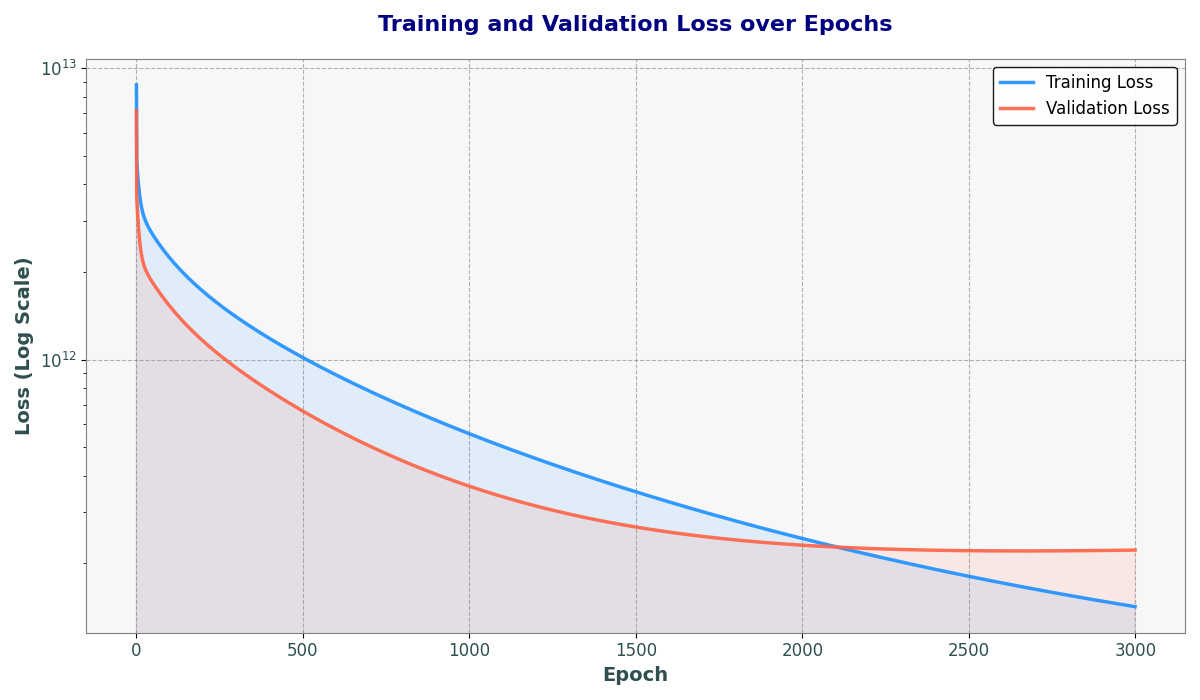
\includegraphics[width=0.9\textwidth]{img_multiple/loss_lasso.png} % Hình lớn chiếm 90% chiều rộng
    \caption{Giá trị hàm mất mát qua từng epoch (Lasso)}
    \label{fig:loss_lasso}
\end{figure}

% Figure 2: Hai subfigure nằm ngang bên dưới
\begin{figure}[H]
    \centering
    \begin{subfigure}[b]{0.48\textwidth}
        \centering
        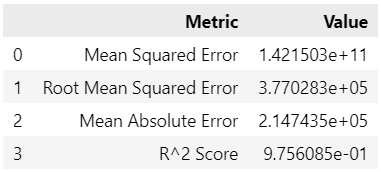
\includegraphics[width=\linewidth]{img_multiple/metrics_lasso_train.png}
        \caption{Đánh giá trên tập huấn luyện}
    \end{subfigure}
    \hfill
    \begin{subfigure}[b]{0.48\textwidth}
        \centering
        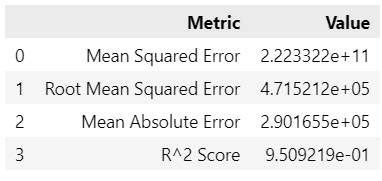
\includegraphics[width=\linewidth]{img_multiple/metrics_lasso_val.png}
        \caption{Đánh giá trên tập kiểm chứng}
    \end{subfigure}
    \caption{So sánh đánh giá mô hình trên tập huấn luyện và kiểm chứng (Lasso)} 
\end{figure}

\paragraph{Hồi quy Ridge (Ridge Regression)}
Phương pháp hồi quy Ridge sử dụng kỹ thuật điều chuẩn L2, đã được giới thiệu ở 2.3.3

\begin{figure}[H]
    \centering
    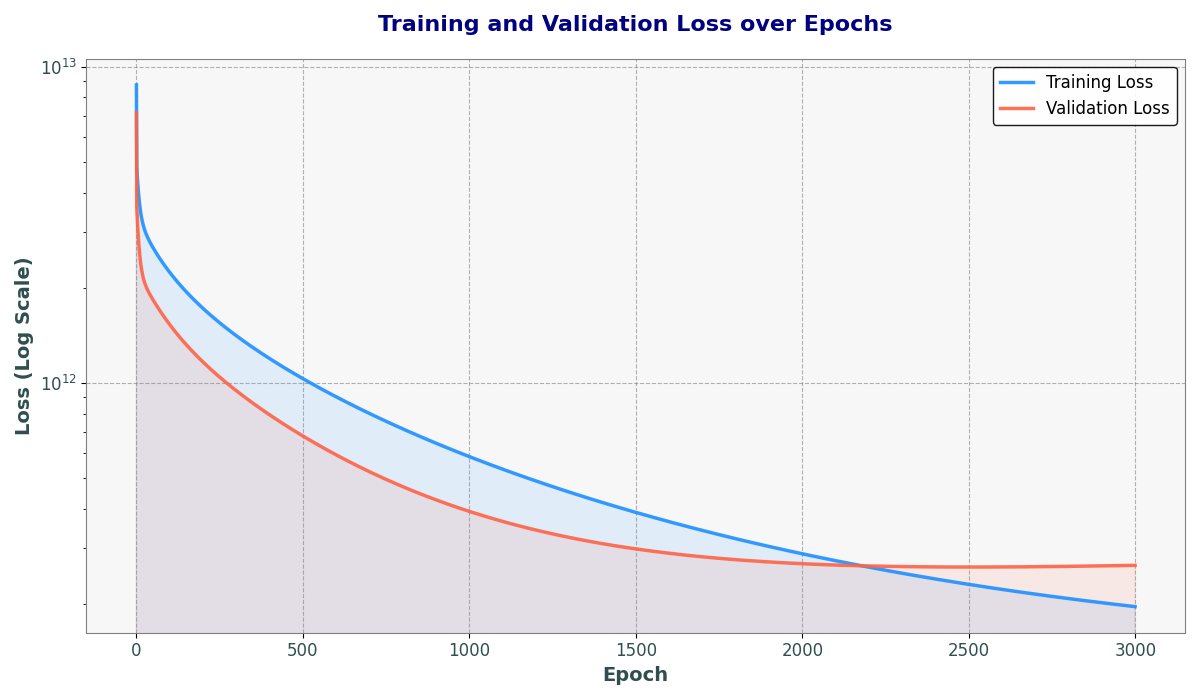
\includegraphics[width=0.9\textwidth]{img_multiple/loss_ridge.png} % Hình lớn chiếm 90% chiều rộng
    \caption{Giá trị hàm mất mát qua từng epoch (Ridge)}
    \label{fig:loss_ridge}
\end{figure}

% Figure 2: Hai subfigure nằm ngang bên dưới
\begin{figure}[H]
    \centering
    \begin{subfigure}[b]{0.48\textwidth}
        \centering
        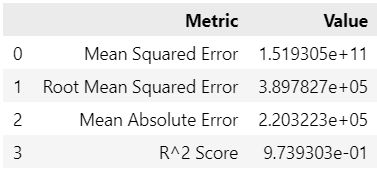
\includegraphics[width=\linewidth]{img_multiple/metrics_ridge_train.png}
        \caption{Đánh giá trên tập huấn luyện}
    \end{subfigure}
    \hfill
    \begin{subfigure}[b]{0.48\textwidth}
        \centering
        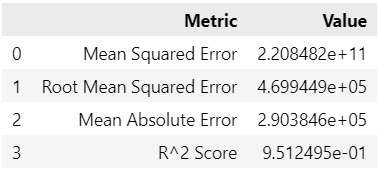
\includegraphics[width=\linewidth]{img_multiple/metrics_ridge_val.png}
        \caption{Đánh giá trên tập kiểm chứng}
    \end{subfigure}
    \caption{So sánh đánh giá mô hình trên tập huấn luyện và kiểm chứng (Ridge)} 
\end{figure}

\subsection{Nhận xét và đánh giá}
\subsubsection{Đánh giá tổng quan hiệu năng mô hình}

Bảng dưới đây trình bày kết quả đánh giá hiệu năng của các mô hình và các phương pháp khác nhau:

\begin{figure}[H]
    \centering
    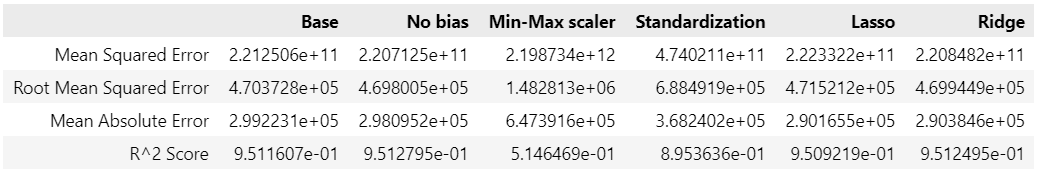
\includegraphics[width=1\linewidth]{img_multiple/summary.png}
    \caption{Tổng kết mức hiệu quả của từng phương pháp}
    \label{fig:summary}
\end{figure}

Phân tích kết quả cho thấy một số điểm đáng chú ý sau:

\begin{enumerate}
    \item \textbf{Về giá trị mất mát:} Các chỉ số MSE (Mean Squared Error) ghi nhận giá trị tương đối cao, lên đến hàng trăm tỷ. Tuy nhiên, điều này không đáng lo ngại vì biến mục tiêu Price vốn có phạm vi giá trị rất lớn. Đặc biệt là với hàm MSE, độ chênh lệch lên cả hàng trăm tỷ vì hàm có bậc bình phương, dẫn đến sẽ đẩy cao giá trị mất mát lên nhiều lần.
    
    \item \textbf{Hiệu suất mô hình cơ sở:} Mô hình cơ sở (Base) và mô hình không thành phần bias (No bias) đều đạt hiệu suất tương đương nhau với chỉ số R$^2$ xấp xỉ 0.951. Điều này cho thấy rằng trong bài toán cụ thể này, thành phần bias không đóng vai trò quan trọng đến hiệu năng của mô hình.
    
    \item \textbf{Tác động của các phương pháp chuyển hóa biến mục tiêu:} Min-Max scaling làm giảm hiệu suất của mô hình đáng kể, với chỉ số R$^2 \approx 0.514$, trong khi đó Standardization đem lại kết quả tương đối tích cực, với R$^2$ đạt gần 0.9
    
    \item \textbf{Hiệu quả của Regularization:} Các phương pháp điều chuẩn (Lasso và Ridge) cho hiệu suất tương đương với mô hình cơ sở (R$^2 \approx 0.951$), chứng tỏ các kỹ thuật regularization có khả năng kiểm soát độ phức tạp của mô hình mà không làm ảnh hưởng đến hiệu suất dự đoán.
\end{enumerate}

\textbf{Kết luận:} Mô hình cơ sở, không bias và các mô hình có áp dụng regularization (Lasso, Ridge) cho hiệu suất xuất sắc với chỉ số R$^2$ đạt 0.951, nghĩa là các mô hình này có khả năng giải thích được 95.1\% phương sai trong dữ liệu giá nhà. Các phương pháp chuyển hóa biến mục tiêu không mang lại cải thiện đáng kể về hiệu suất trong bài toán này, thậm chí còn làm giảm khả năng dự đoán của mô hình.

\subsubsection{Vấn đề với việc chuyển hóa biến mục tiêu}
Tùy thuộc vào bài toán, việc scale biến mục tiêu có thể gia tăng hiệu suất mô hình lên đáng kể (tốc độ học nhanh hơn, tiết kiệm chi phí,...). Theo như thống kê [\ref{fig:summary}], Min-Max scaling đem lại kết quả khá tệ. Lý do có thể là một vài nguyên nhân chính sau đây:

\begin{itemize}
    \item \textbf{Min-Max Scaling}: Phương pháp này đưa biến mục tiêu về khoảng [0,1], giữ nguyên dạng phân phối nhưng nén phạm vi giá trị. Việc nén này có thể làm mất thông tin về không gian giữa các đặc trưng, dẫn đến mô hình học sai các mối quan hệ.

    \begin{figure}[H]
        \centering
        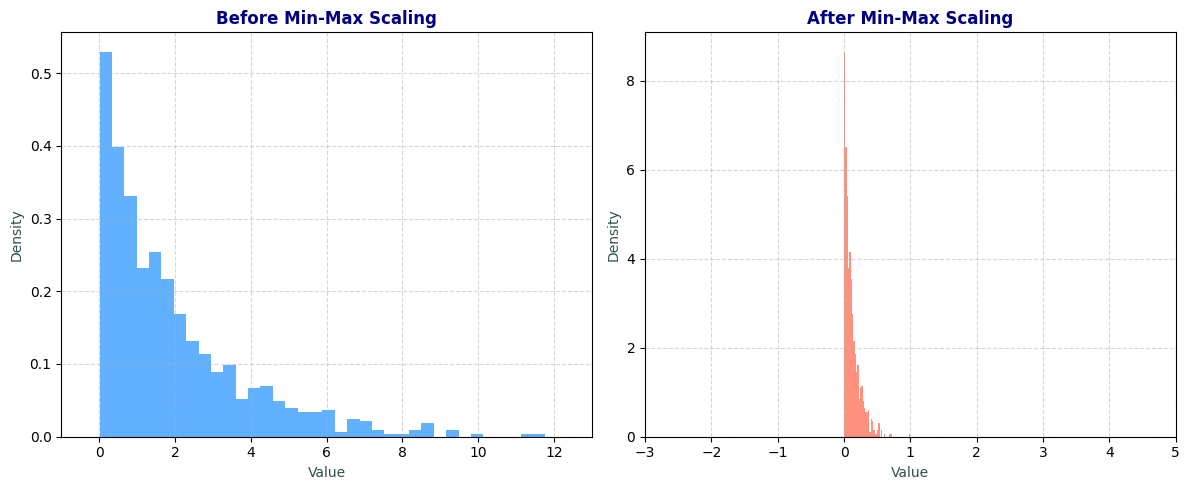
\includegraphics[width=1\linewidth]{img_multiple/output_min_max.png}
        \caption{Minh họa phân phối dữ liệu trước và sau Min-Max Scaling}
    \end{figure}

    \textit{Nhận xét:} Dễ thấy độ phân tán của các điểm dữ liệu thấp do bị ép nén về một phạm vi nhỏ.
    
    \item \textbf{So sánh với Standardization}: Ngược lại, Standardization hoạt động hiệu quả hơn vì đây là một phép biến đổi tuyến tính, nó không làm thay đổi mối quan hệ tuyến tính giữa biến đầu vào và đầu ra, đồng thời, nó vần đưa biến mục tiêu về cùng thang đo với các đặc trưng đã chuẩn hóa, giúp cải thiện hiệu suất.

    \begin{figure}[H]
        \centering
        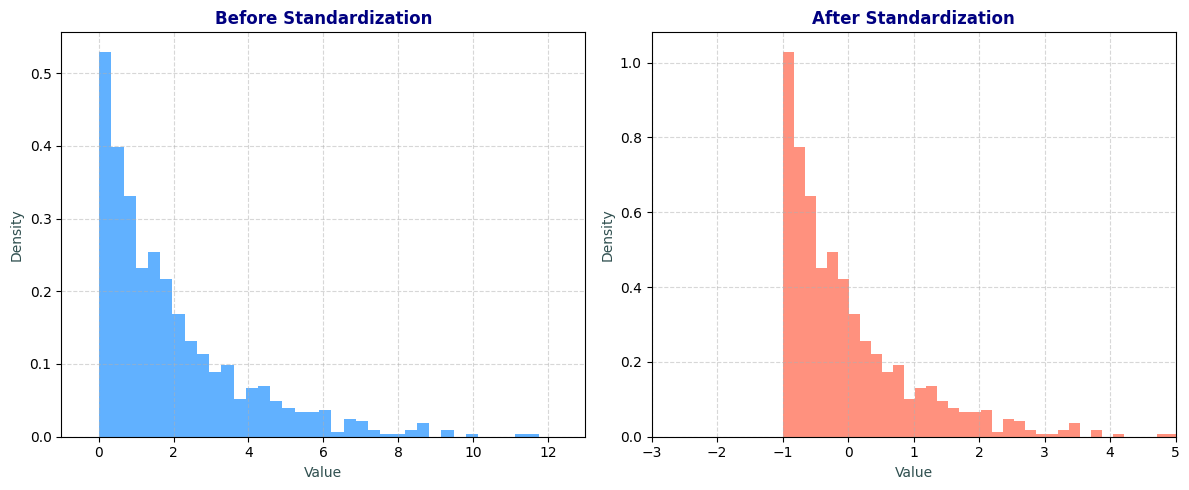
\includegraphics[width=1\linewidth]{img_multiple/output_standard.png}
        \caption{Minh họa phân phối dữ liệu trước và sau Standardization}
    \end{figure}
\end{itemize}

\subsubsection{Kết quả dự đoán của mô hình tốt nhất:}

\begin{figure}[H]
    \centering
    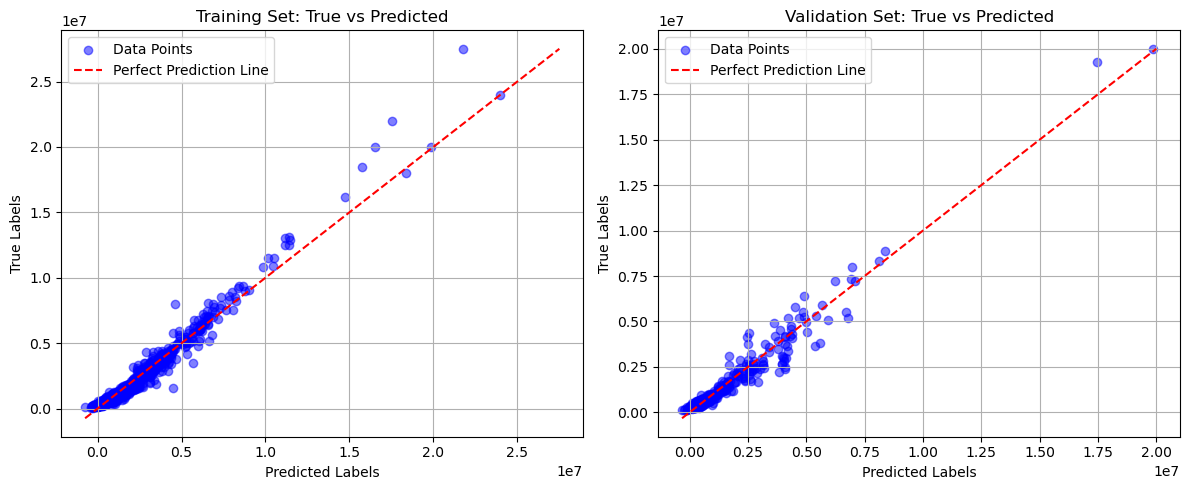
\includegraphics[width=1\linewidth]{img_multiple/output_final.png}
    \caption{Đường thẳng hồi quy dự đoán so với thực tế, trên tập huấn luyện và kiểm chứng}
    \label{fig:enter-label}
\end{figure}

\pagebreak % 0
\newpage
\section{Mô hình hồi quy tuyến tính đa thức}

\paragraph{}{\textbf{Hồi quy tuyến tính đa thức} \cite{ostertagova2012modelling} (Polynomial regression) là một dạng hồi quy mở rộng của hồi quy tuyến tính, trong đó mối quan hệ giữa biến độc lập và biến phụ thuộc không phải là một đường thẳng mà là một đa thức bậc cao hơn. Ngoài ra, hồi quy tuyến tính đa thức còn là mô hình hiệu quả để đánh giá các mối quan hệ phi tuyến tính giữa các giá trị đầu vào và đầu ra, đặc biệt hữu dụng khi phân loại các dữ liệu cần đường hồi quy phức tạp.}

\paragraph{}{Với hồi quy tuyến tính đa thức, mô hình được mở rộng thành các bậc cao hơn của biến độc lập X. Mô hình hồi quy đa thức đơn biến bậc n có dạng:}

\begin{center}
\large $Y = \beta_0+\beta_1*X+\beta_2*X^2+...+\beta_k*X^k + \epsilon$
\end{center}

Trong đó:
\begin{itemize}
    \item $k$: Bậc của đa thức
    \item $X$: Biến độc lập
    \item $Y$: Biến phụ thuộc
    \item $\epsilon$: Thành phần sai số
    \item $\beta_0$: Hệ số chặn (intercept)
    \item $\beta_1,\beta_2...,\beta_k$: Các hệ số hồi quy (coefficient)
\end{itemize}

\subsection{Xây dựng mô hình}
\subsubsection{Phương pháp xây dựng}

\paragraph{}{Nếu coi mỗi lũy thừa của biến độc lập như một biến độc lập mới: $X_1 = X, X_2 = X^2, X_3 = X^3, ...$. Ta nhận thấy rằng mô hình hồi quy đa thức trở thành:}

\begin{center}
\large $Y = \beta_0+\beta_1*X_1+\beta_2*X_2+...+\beta_k*X_k + \epsilon$
\end{center}

\paragraph{}{Nhận xét: Qua mô hình trên thấy được hồi quy tuyến tính đa thức là một dạng đặc biệt của hồi quy tuyến tính đa biến (Multiple Linear Regression) (xem ở \ref{label:lr}). Vì vậy để xây dựng mô hình hồi quy tuyến tính đa thức, ta có thể xây dựng dựa vào mô hình hồi quy đa biến với các đặc trưng đa thức $[X, X^1, X^2,X^3,...,X^k]$.}

\paragraph{}{Ta sử dụng \textbf{phương pháp bình phương tối thiểu} (Ordinary Least Squares - OLS) (xem \ref{label:simple-linear}) hoặc \textbf{phương pháp Gradient Descent} (xem \ref{label:GradientDecent}) để giải quyết bài toán. Ngoài ra, ta có thể sử dụng thêm kỹ thuật \textbf{Chính quy hóa} (Regularization) với L1 (Lasso) (xem \ref{label:lasso-math}) hoặc L2 (Ridge) (xem \ref{label:ridge-math}) để giảm tình trạng overfitting hoặc giải được bài toán hồi quy đa thức bậc cao với nhiều đặc trưng (đa biến) có bao gồm sự tương tác giữa các đặc trưng với nhau.}

\subsubsection{Xây dựng đặc trưng đa thức}
\paragraph{a) Giới thiệu:}{Đặc trưng đa thức là các đặc trưng mới được xây dựng từ các đặc trưng đầu vào gốc bằng cách nâng bậc chúng lên. Ví dụ:}
\paragraph{}{Với một biến đầu vào x:}
\begin{itemize}
    \item Bậc 1: $x$ (đặc trưng gốc)
    \item Bậc 2: $x, x^2$
    \item Bậc 3: $x, x^2, x^3$
    \item ...
    \item Bậc k: $x, x^2, x^3, ..., x^k$
\end{itemize}
\paragraph{}{Với hai biến đầu vào $x_1$ và $x_2$ (Bao gồm sự tương tác giữa các biến):}
\begin{itemize}
    \item Bậc 1: $x_1, x_2$ (đặc trưng gốc)
    \item Bậc 2: $x_1, x_2, x_1^2, x_2^2, x_1*x_2$
    \item Bậc 3: $x_1, x_2, x_1^2, x_2^2, x_1*x_2, x_1^3, x_2^3, x_1^2*x_2, x_1*x_2^2$
    \item ...
\end{itemize}
\paragraph{}{Tương tự với các trường hợp biến đầu vào nhiều hơn 2. Vì vậy sau khi áp dụng biến đổi đa thức với bậc d, chúng ta sẽ thu được ma trận đặc trưng đa thức $X_{poly}$ với kích thước $n*m$, trong đó m là số lượng đặc trưng đa thức được tạo ra tính bằng công thức dưới.}

\paragraph{b) Công thức tính tổng quát số lượng đặc trưng đa thức:}{}
\begin{center}
\large $C(k + d, d) = \binom{k + d}{d} = \frac{(k + d)!}{d! * k!}$
\end{center}
Trong đó:
\begin{itemize}
    \item $C(k + d, d)$: tổ hợp chập $d$ của $k + d$.
    \item $k$: số lượng biến đầu vào (features) ban đầu.
    \item $d$: bậc đa thức tối đa.
\end{itemize}

\paragraph{c) Ma trận hóa:}{Quá trình ma trận hóa đặc trưng đa thức thực hiện biến đổi trên từng hàng (mẫu) của ma trận đầu vào $\mathbf{X}$ để tạo ra một hàng mới trong ma trận $\mathbf{X_{poly}}$.}

\paragraph{}{Ví dụ minh họa với 2 biến đầu vào (k=2) và bậc đa thức d=2:}

\paragraph{}{Giả sử chúng ta có một mẫu dữ liệu duy nhất $\mathbf{x} = \begin{pmatrix} x_1 & x_2 \end{pmatrix}$ và chúng ta muốn tạo đặc trưng đa thức bậc 2. Các đặc trưng đa thức được tạo ra là:}

\begin{enumerate}
    \item Bậc 0: $1$ (bias term)
    \item Bậc 1: $x_1, x_2$
    \item Bậc 2: $x_1^2, x_1x_2, x_2^2$
\end{enumerate}

\paragraph{}{Như vậy, vector đặc trưng đa thức cho mẫu $\mathbf{x}$ sẽ là:}

$$
\mathbf{x_{poly}} = \begin{pmatrix} 1 & x_1 & x_2 & x_1^2 & x_1x_2 & x_2^2 \end{pmatrix}
$$

\paragraph{}{Tổng quát hóa cho ma trận X:}

\paragraph{}{Để tạo ma trận $\mathbf{X_{poly}}$ từ ma trận $\mathbf{X}$, chúng ta sẽ áp dụng biến đổi trên cho từng hàng của $\mathbf{X}$.\newline

Ví dụ, nếu ma trận đầu vào $\mathbf{X}$ là:}

$$
\mathbf{X} =
\begin{pmatrix}
  x_{11} & x_{12} \\
  x_{21} & x_{22} \\
  x_{31} & x_{32}
\end{pmatrix}
$$

\paragraph{}{Thì ma trận đặc trưng đa thức $\mathbf{X_{poly}}$ bậc 2 sẽ là:}

$$
\mathbf{X_{poly}} =
\begin{pmatrix}
  1 & x_{11} & x_{12} & x_{11}^2 & x_{11}x_{12} & x_{12}^2 \\
  1 & x_{21} & x_{22} & x_{21}^2 & x_{21}x_{22} & x_{22}^2 \\
  1 & x_{31} & x_{32} & x_{31}^2 & x_{31}x_{32} & x_{32}^2
\end{pmatrix}
$$

\paragraph{}{Dựa trên ma trận hóa của mô hình \textbf{hồi quy đa biến (Multiple Regression)} (xem \ref{label:simple-linear}). Đối với toàn tập dữ liệu có $n$ quan sát và $m$ đặc trưng đa thức (features), ta có thể biểu diễn tổng quát ma trận hồi quy:}

\begin{equation}
    \begin{bmatrix}
        y_1 \\
        y_2 \\
        \vdots \\
        y_n
    \end{bmatrix}
    _{\text{$n \times 1$}}
    = 
    \begin{bmatrix}
        1 & x_{11} & x_{12} & \dots & x_{11}^2 & x_{12}^2 & \dots & x_{11} \cdot x_{12} & \dots\\
        1 & x_{21} & x_{22} & \dots & x_{21}^2 & x_{22}^2 & \dots & x_{21} \cdot x_{22} & \dots \\
        \vdots & \vdots & \vdots & \ddots & \vdots & \vdots & \ddots & \vdots & \ddots \\
        1 & x_{n1} & x_{n2} & \dots & x_{n1}^2 & x_{n2}^2 & \dots & x_{n1} \cdot x_{n2} & \dots \\
    \end{bmatrix}
    _{\text{$n \times m$}}
    \begin{bmatrix}
        \beta{0} \\
        \beta{1} \\
        \vdots \\
        \beta{m}
    \end{bmatrix}
    _{\text{$m \times 1$}}
    +
    \begin{bmatrix}
        \epsilon_{1} \\
        \epsilon_{2} \\
        \vdots \\
        \epsilon_{n}
    \end{bmatrix}
    _{\text{$n \times 1$}}
\end{equation}

\paragraph{}{Phương trình này có thể được biểu diễn một cách ngắn gọn hơn trong ký hiệu ma trận:}

\begin{equation}
    \mathbf{Y} = \mathbf{X_{poly}}\boldsymbol{\beta} + \epsilon
\end{equation}

Trong đó:
\begin{itemize}
    \item $\mathbf{Y} \in \mathbb{R}^{n \times 1}$ là vector cột chứa $n$ giá trị phụ thuộc
    \item $\mathbf{X} \in \mathbb{R}^{n \times m}$ là ma trận chứa $n$ mẫu quan sát với $m$ đặc trưng đa thức cho mỗi mẫu
    \item $\boldsymbol{\beta} \in \mathbb{R}^{m \times 1}$ là vector hệ số hồi quy cần ước lượng
    \item $\epsilon \in \mathbb{R}^{n \times 1}$ là giá trị thành phần sai số ngẫu nhiên (the random error component)
\end{itemize}

\paragraph{d) Nhận xét:}{Bậc của đa thức là một hyperparameter quan trọng trong hồi quy đa thức. Việc lựa chọn bậc phù hợp có ảnh hưởng lớn đến hiệu suất của mô hình:}
\begin{itemize}
    \item Bậc quá thấp (Underfitting): Mô hình quá đơn giản, không thể nắm bắt được các mẫu phức tạp trong dữ liệu. Dẫn đến sai số cao trên cả dữ liệu huấn luyện và dữ liệu kiểm tra.

    \item Bậc vừa phải (Good Fit): Mô hình có độ phức tạp vừa đủ để nắm bắt được các mẫu quan trọng trong dữ liệu mà không quá khớp. Đạt được hiệu suất tốt trên cả dữ liệu huấn luyện và dữ liệu kiểm tra.

    \item Bậc quá cao (Overfitting): Mô hình quá phức tạp, khớp quá sát với dữ liệu huấn luyện, bao gồm cả nhiễu. Dẫn đến sai số thấp trên dữ liệu huấn luyện nhưng sai số cao trên dữ liệu kiểm tra (khả năng tổng quát hóa kém).
\end{itemize}

\subsubsection{Huấn luyện mô hình}
\paragraph{}{Để huấn luyện mô hình \textbf{hồi quy đa thức (Polynomial Regression)} ta có thể sử dụng quá trình huấn luyện mô hình bằng phương pháp Gradient Descent của \textbf{hồi quy đa biến (Multiple Regression)} (xem \ref{label:GradientDecent}) dựa trên đặc trưng đa thức được xây dựng ở trên.}

\paragraph{}{\textbf{Các tham số:}}
\begin{itemize}
    \item Learning rate: 0.01
    \item Số epoch: 5000
    \item Batch size: 32
    \item Epsilon: $10^{-8}$ (Ngưỡng hội tụ)
\end{itemize}

\paragraph{}{\textbf{Triển khai:}}
\begin{itemize}
    \item Dữ liệu huấn luyện được sắp xếp ngẫu nhiên trước mỗi epoch để giảm thiểu phương sai trong quá trình cập nhật trọng số.
    \item Batch Gradient Descent được sử dụng để cập nhật trọng số mô hình.
    \item Lưu lại bộ trọng số tốt nhất trong quá trình huấn luyện.
\end{itemize}

\paragraph{}{\textbf{Quá trình huấn luyện:}}

\begin{figure}[H]
    \centering
    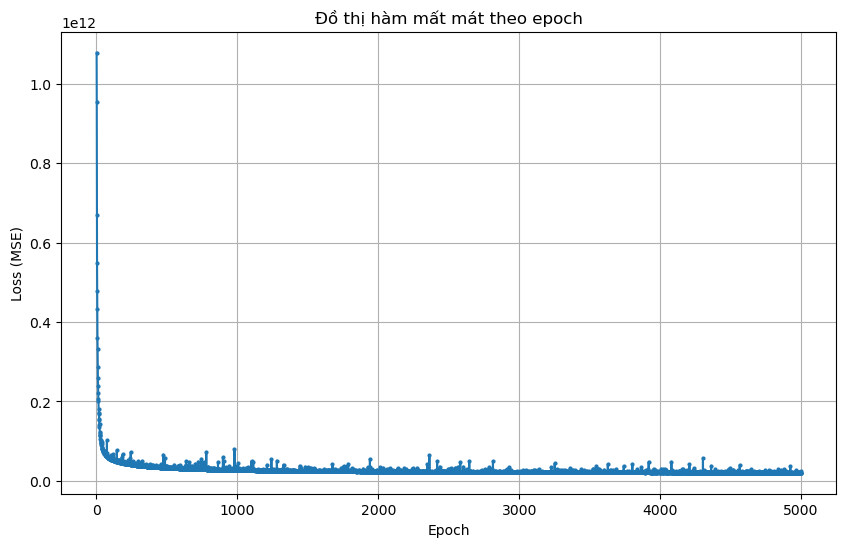
\includegraphics[width=0.7\textwidth]{img/Poly_Loss_Plot.png}
    \caption{Biểu đồ Loss qua các Epoch.}
    \label{fig:poly-loss_plot}
\end{figure}

\begin{itemize}
    \item Biểu đồ cho thấy giá trị hàm mất mát (Loss) giảm dần theo số epoch, chứng tỏ mô hình đang học được các mẫu từ dữ liệu huấn luyện.
    \item Ban đầu, loss rất lớn (khoảng hơn $10^{12}$), nhưng sau 5000 epoch, nó giảm xuống đáng kể còn khoảng $2 * 10^{10}$.
    \item Mô hình đạt được giá trị loss tối ưu (trên tập huấn luyện là $20342161463.87$)
\end{itemize}

\subsubsection{Công thức hồi quy}
\paragraph{}{Hiển thị top 10 số hạng dựa trên hệ số hồi quy lớn nhất:}

\begin{center}
\small $Price = 1680790.7703 \cdot Model + 1559994.1677 \cdot Model \cdot Year + 1464639.3648 \cdot Model \cdot Year^2 + 1046459.7736 \cdot Model \cdot Transmission + 1046459.7736 \cdot Model \cdot Transmission^2 + 1009863.5419 \cdot Model \cdot Kilometer + 946888.0919 \cdot Model \cdot Year \cdot Transmission + 938621.1008 \cdot Model \cdot Location + 938621.1008 \cdot Model \cdot Location^2 + 935093.6800 \cdot Model \cdot Year \cdot Kilometer + ...$
\end{center}

Trong đó:
\begin{itemize}
    \item $Price$: Giá xe được dự đoán bởi mô hình
    \item $Model, Year, Transmission, ...$: Giá trị của các đặc trưng trong tập dữ liệu sau các quá trình xử lí dữ liệu.
\end{itemize}

Nhận xét: Dựa vào công thức hồi quy, ta thấy \texttt{Model} là đặc trưng tốt nhất có khả năng tương quan thuận với \texttt{Price}. Ngoài ra, các đặc trưng như \texttt{Year}, \texttt{Tranmission} cũng có sự ảnh hưởng lớn đến giá trị \texttt{Price}.

\subsection{Đánh giá mô hình}

\begin{figure}[H]
    \centering
    \begin{subfigure}[b]{0.48\textwidth}
        \centering
        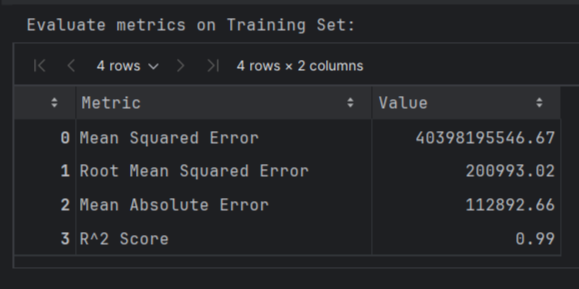
\includegraphics[width=\linewidth]{img/Evaluate_Poly_Training_Set.png}
        \caption{Đánh giá trên tập huấn luyện}
        \label{fig:poly-linear-train}
    \end{subfigure}
    \hfill
    \begin{subfigure}[b]{0.48\textwidth}
        \centering
        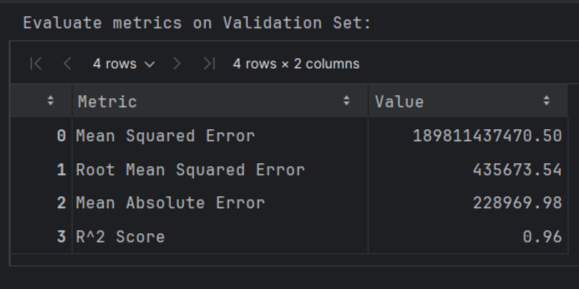
\includegraphics[width=\linewidth]{img/Evaluate_Poly_Validation_Set.png}
        \caption{Đánh giá trên tập kiểm chứng}
        \label{fig:poly-linear-valid}
    \end{subfigure}
    \caption{So sánh đánh giá mô hình hồi quy đa thức bậc 3 trên tập huấn luyện và kiểm chứng} 
    \label{fig:poly-linear-eval}
\end{figure}

\paragraph{}{Trên tập huấn luyện, mô hình đạt MSE là $40398195546.67 \approx 4.0398 * 10^{10}$ và R² là $0.99$, cho thấy mô hình rất khớp với dữ liệu đã thấy. Tuy nhiên, trên tập kiểm chứng, MSE tăng lên đáng kể thành $189811437470.50 \approx 1.8981 * 10^{11}$ và R² giảm xuống còn $0.96$.}

\paragraph{}{Mặc dù giá trị R² trên tập kiểm chứng vẫn khá cao, sự gia tăng đáng kể của các chỉ số lỗi (MSE tăng gấp $5$ lần, RMSE và MAE tăng gấp $2$ lần) cho thấy dấu hiệu của hiện tượng overfitting. Mô hình đã học thuộc một số đặc điểm nhiễu của tập huấn luyện và khả năng tổng quát hóa trên dữ liệu mới bị hạn chế hơn. Điều này cũng có thể quan sát thấy trong hình \ref{fig:poly-linear-eval}, nơi các điểm dữ liệu kiểm chứng phân tán rộng hơn quanh đường dự đoán so với tập huấn luyện.}

\begin{figure}[H]
    \centering
    \begin{subfigure}[b]{1\textwidth} % Tăng chiều rộng lên để ảnh chiếm gần hết chiều rộng trang
        \centering
        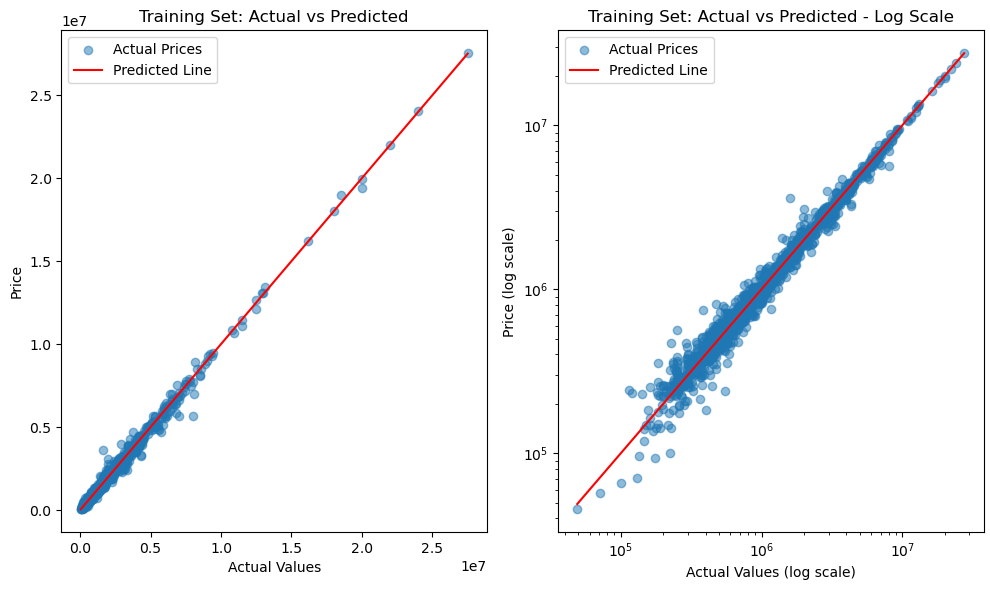
\includegraphics[width=\linewidth]{img/Poly_Training_Plot.png}
        \caption{Đánh giá trên tập huấn luyện}
        \label{fig:poly-linear-train-plot}
    \end{subfigure}

    \begin{subfigure}[b]{1\textwidth} % Tăng chiều rộng lên để ảnh chiếm gần hết chiều rộng trang
        \centering
        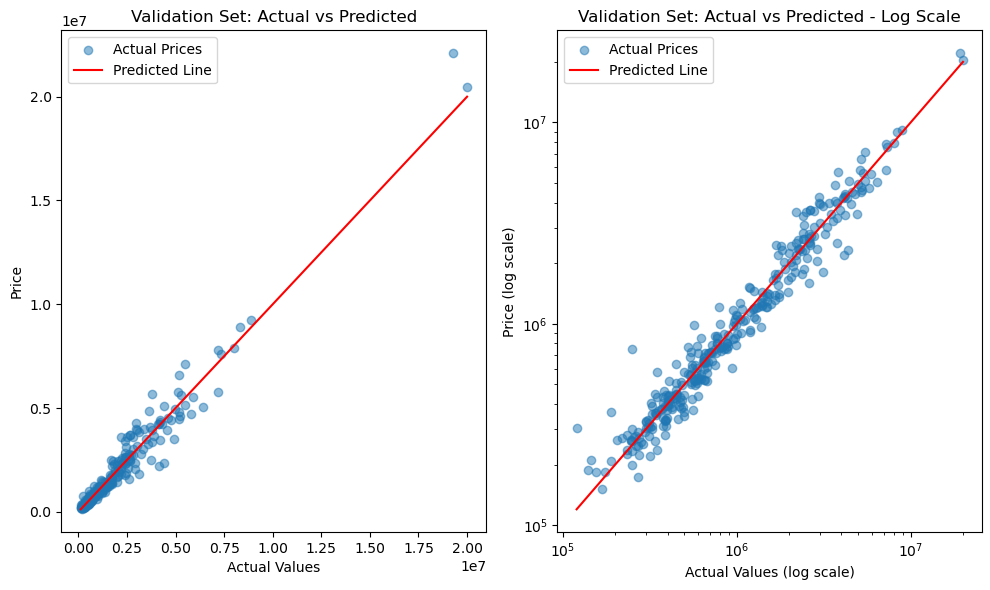
\includegraphics[width=\linewidth]{img/Poly_Validation_Plot.png}
        \caption{Đánh giá trên tập kiểm chứng}
        \label{fig:poly-linear-valid-plot}
    \end{subfigure}
    \caption{So sánh đánh giá mô hình hồi quy đa thức bậc 3 trên tập huấn luyện và kiểm chứng}
    \label{fig:poly-linear-eval-plot}
\end{figure}

\pagebreak

 % ?
\newpage
\section{Mô hình hồi quy tuyến tính kết hợp với các phương pháp PCA(Principal Component Analysis)}

\paragraph{}{PCA (Principal Component Analysis) giúp giảm chiều dữ liệu bằng cách tìm ra các \textbf{thành phần chính (Principal Components - PCs)} mà vẫn giữ được nhiều thông tin nhất. Trong tập dữ liệu này, ta có nhiều biến liên quan đến nhau (tương quan cao), nên việc dùng PCA giúp:}

\begin{itemize}
    \item \textbf{Giảm đa cộng tuyến} (nhiều biến có tương quan cao sẽ gây khó khăn cho mô hình dự đoán).
    \item \textbf{Tăng hiệu suất tính toán} (mô hình không cần xử lý quá nhiều biến).
    \item \textbf{Loại bỏ nhiễu} và \textbf{giữ lại thông tin quan trọng} nhất.
\end{itemize}

\subsection{Phân tích tương quan và chọn nhóm biến}
\label{subsec:correlation}

\begin{figure}[H] 
    \centering
    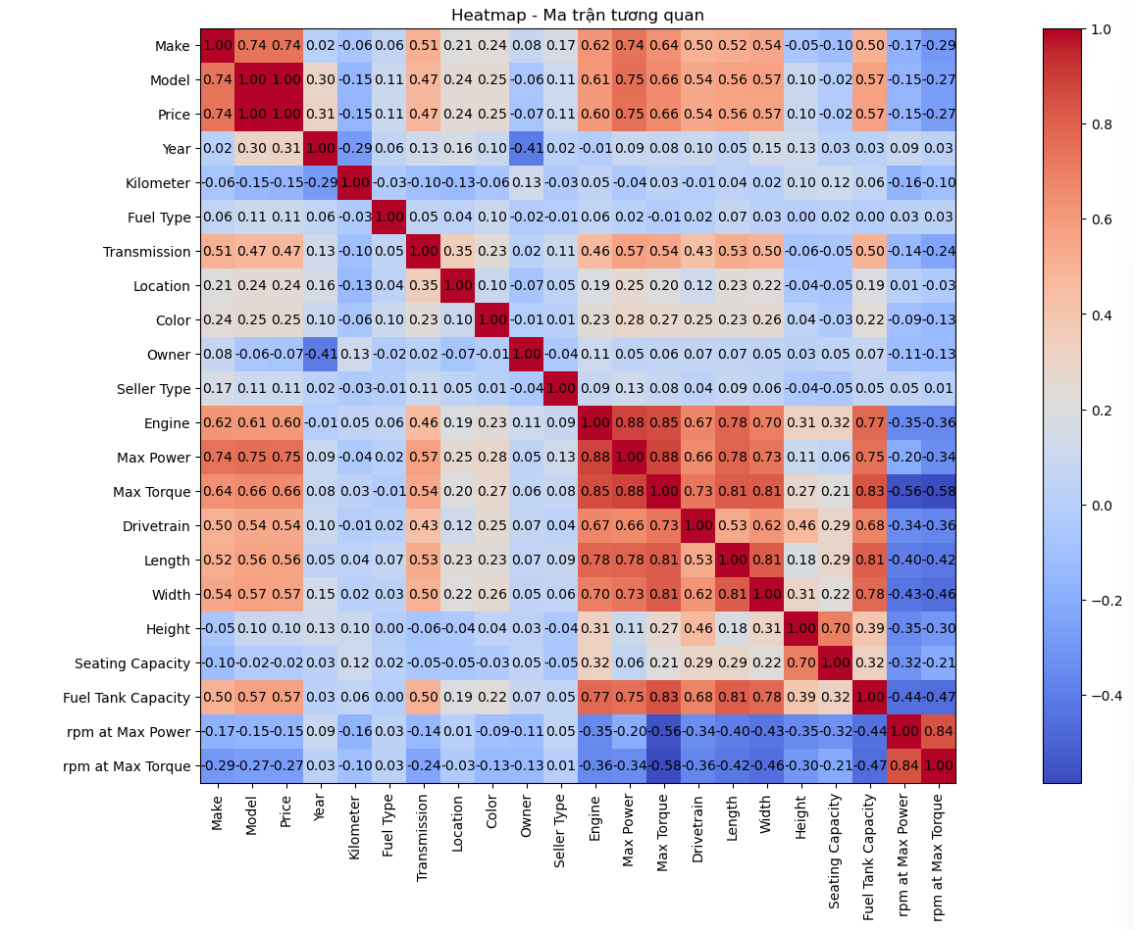
\includegraphics[width=1\textwidth]{img/heatmapPCA.png} 
    \caption{Ma trận tương quan giữa các biến.}
    \label{fig:correlation_matrix}
\end{figure}

\paragraph{}{Phân tích ma trận tương quan cho thấy các nhóm biến có mối liên hệ chặt chẽ:}
\begin{itemize}
    \item \textbf{Nhóm kích thước xe} (\texttt{Seating Capacity}, \texttt{Length}, \texttt{Height}, \texttt{Width}, \texttt{Fuel Tank Capacity}) có mối tương quan cao, đặc biệt giữa \texttt{Length} - \texttt{Width} (0.81), \texttt{Height} - \texttt{Seating Capacity} (0.7) và \texttt{Fuel Tank Capacity} - \texttt{Width} (0.78), cho thấy khả năng giảm chiều dữ liệu.
    \item \textbf{Nhóm công suất động cơ} (\texttt{Engine}, \texttt{Max Power}, \texttt{Max Torque}, \texttt{Drivetrain}) có quan hệ chặt chẽ, với \texttt{Engine} - \texttt{Max Power} (0.88) và \texttt{Max Power} - \texttt{Max Torque} (0.88). \texttt{Drivetrain} - \texttt{Max Torque} (0.72) cho thấy khả năng giảm chiều dữ liệu.
    \item \textbf{Nhóm vòng tua động cơ} (\texttt{rpm at Max Power}, \texttt{rpm at Max Torque}) có tương quan 0.84, thể hiện mối quan hệ tuyến tính mạnh, phù hợp để giảm số chiều dữ liệu.
\end{itemize}

\subsection{Áp dụng phương pháp PCA}
\label{label: PCA}
\label{subsec:apply_pca}

\paragraph{}{PCA được áp dụng trên ba nhóm biến có tương quan cao nhằm giảm chiều dữ liệu mà vẫn bảo toàn thông tin quan trọng. Quá trình thực hiện gồm các bước:}

\begin{enumerate}
    \item \textbf{Áp dụng PCA trên tập train}:
    \begin{itemize}
        \item Áp dụng phương pháp PCA (xem các bước thực hiện ở \ref{label: pca})
        \item Kết quả thu được ba đặc trưng mới: \texttt{PCA\_hs}, \texttt{PCA\_cs}, \texttt{PCA\_kt}.
        \item Các cột ban đầu được loại bỏ khỏi tập dữ liệu.
    \end{itemize}
    \item \textbf{Áp dụng PCA trên tập validation}:
    \begin{itemize}
        \item Sử dụng giá trị trung bình và vector thành phần chính từ tập train để biến đổi dữ liệu validation, đảm bảo nhất quán.
        \item Thay thế các biến gốc bằng các đặc trưng PCA tương ứng.
    \end{itemize}
\end{enumerate}

\paragraph{}{Sau khi áp dụng \textbf{PCA}, ta thu được các 13 đặc trưng gồm \texttt{PCA\_hs}, \texttt{PCA\_cs}, \texttt{PCA\_kt}, cùng với các đặc trưng ban đầu như \texttt{Make}, \texttt{Model}, \texttt{Year}, \texttt{Kilometer}, \texttt{Fuel Type}, \texttt{Transmission}, \texttt{Location}, \texttt{Color}, \texttt{Owner}, \texttt{Seller Type} dùng dể dự đoán giá xe $Price$}

\label{sec:training_evaluation}

\subsection{Chuẩn hóa dữ liệu và chia tập dữ liệu để huấn luyện}
\label{subsec:preprocessing}

\begin{itemize}
    \item \textbf{Chuẩn hóa dữ liệu} bằng phương pháp Z-score (xem \ref{label:standart scaler}). Việc này giúp đưa dữ liệu về cùng một thang đo, giảm ảnh hưởng của đơn vị đo khác nhau và cải thiện tốc độ hội tụ của thuật toán tối ưu (xem \ref{label:toc do hoi tu}).
    % (chứng minh phần Tốc độ Gradient decent khi đưa về ) % -> Có thể thêm tham chiếu đến phụ lục hoặc phần khác nếu có
    \item \textbf{Chia tập dữ liệu}:
    \begin{itemize}
        \item $X_{\text{train\_v2}}$, $X_{\text{val\_v2}}$: Đặc trưng đầu vào (sau chuẩn hóa và PCA).
        \item $y_{\text{train\_v2}}$, $y_{\text{val\_v2}}$: Biến mục tiêu (\texttt{Price}).
    \end{itemize}
\end{itemize}

\subsection{Xây dựng mô hình}
\label{subsec:model_building}
\subsubsection{Phương pháp xây dựng}
\paragraph{}{Mô hình hồi quy tuyến tính đa biến (Multiple Linear Regression) (xem ở \ref{label:lr}) được xây dựng để dự đoán giá xe dựa trên các đặc trưng đã xử lý (bao gồm các thành phần từ PCA và các biến khác).}

\subsubsection{Huấn luyện mô hình}


\paragraph{}{\textbf{Các siêu tham số:}}
\begin{itemize}
    \item Learning rate: 0.001
    \item Số epoch: 200
    \item Batch size: 32
\end{itemize}

\paragraph{}{\textbf{Triển khai:}}
\begin{itemize}
    \item Dữ liệu huấn luyện được xáo trộn trước mỗi epoch để giảm thiểu phương sai trong quá trình cập nhật trọng số.
    \item Batch Gradient Descent được sử dụng để cập nhật trọng số mô hình.
    \item Lưu lại bộ trọng số tốt nhất trong quá trình huấn luyện.
\end{itemize}

\paragraph{}{\textbf{Quá trình huấn luyện:}}

\begin{figure}[H]
    \centering
    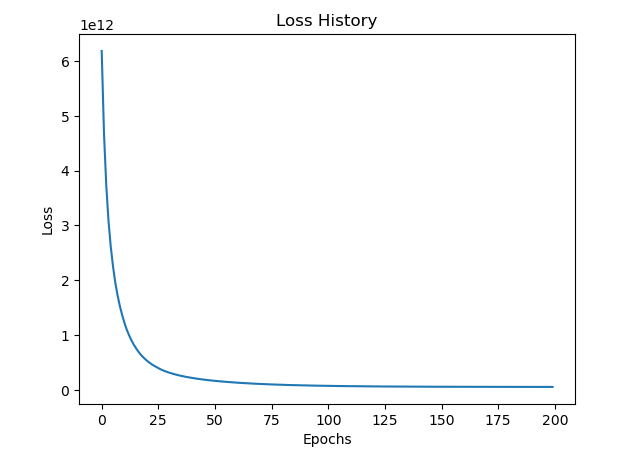
\includegraphics[width=0.7\textwidth]{img/lossPCA.png} % Điều chỉnh width nếu cần
    \caption{Biểu đồ Loss qua các Epoch.}
    \label{fig:loss_plot}
\end{figure}

\begin{itemize}
    \item Biểu đồ cho thấy giá trị hàm mất mát (Loss) giảm dần theo số epoch, chứng tỏ mô hình đang học được các mẫu từ dữ liệu huấn luyện.
    \item Ban đầu, loss rất lớn (khoảng $1369526006662$), nhưng sau 200 epoch, nó giảm xuống đáng kể còn khoảng $552622539599.0718$.
    \item Mô hình đạt được giá trị loss tối ưu (trên tập huấn luyện là $552622539599.0718$)
\end{itemize}
\subsubsection{Công thức hồi quy}
\[
\begin{aligned}
Price = 1715141.18 &+ 57577.71 x_1 + 2332775.74 x_2 + 39443.65 x_3 \\
              &- 7834.82 x_4 + 1770.64 x_5 - 11278.79 x_6 \\
              &- 3295.49 x_7 - 4708.11 x_8 - 18789.88 x_9 \\
              &+ 7566.50 x_{10} + 11094.97 x_{11} - 7151.10 x_{12} \\
              &- 4041.87 x_{13}
\end{aligned}
\]
\paragraph{}{Trong đó:}
\begin{itemize}
    \item $Price$: Giá xe được dự đoán bởi mô hình
    \item $x_i$ với $i \in \{1, 2, \dots, 13\}$: Giá trị của các đặc trưng sau các quá trình xử lí dữ liệu và quá trình PCA (xem \ref{label: PCA})
\end{itemize}
\subsection{Đánh giá mô hình}

\begin{figure}[H]
    \centering
    \begin{subfigure}[b]{0.445\textwidth}
        \centering
        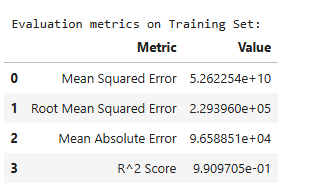
\includegraphics[width=\linewidth]{img/metrictrainPCA.png}
        \caption{Đánh giá trên tập huấn luyện}
        \label{fig:PCA-linear-train}
    \end{subfigure}
    \hfill
    \begin{subfigure}[b]{0.48\textwidth}
        \centering
        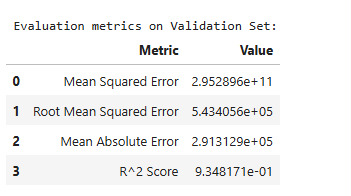
\includegraphics[width=\linewidth]{img/metricvalPCA.png}
        \caption{Đánh giá trên tập kiểm chứng}
        \label{fig:PCAlinear-valid}
    \end{subfigure}
    \caption{So sánh đánh giá mô hình trên tập huấn luyện và kiểm chứng} 
    \label{fig:PCA-linear-eval}
\end{figure}
\paragraph{}{
Trên tập huấn luyện, mô hình đạt MSE là \( 5.262254 \times 10^{10} \) và \( R^2 \) là \( 0.9910 \) (từ \( 9.909705e-01 \)), cho thấy mô hình đã học tốt giữa biến đầu vào biến đầu ra. Tuy nhiên, trên tập kiểm chứng, MSE tăng lên đáng kể thành \( 2.952896 \times 10^{11} \) và \( R^2 \) giảm xuống còn \( 0.9348 \) (từ \( 9.348171e-01 \)).

Mặc dù \( R^2 \) trên tập kiểm chứng vẫn khá cao, sự gia tăng đáng kể của các chỉ số lỗi (MSE tăng từ \( 5.26 \times 10^{10} \) lên \( 2.95 \times 10^{11} \)) cho thấy dấu hiệu của hiện tượng overfitting. Điều này cho thấy rằng mô hình đã học quá tốt trên bộ dữ liệu, làm giảm khả năng tổng quát hóa trên bộ dữ liệu mới.

Biểu đồ “Actual vs Predicted” minh họa sự so sánh giữa giá trị thực tế và giá trị dự đoán của mô hình (quan sát thấy trong hình \ref{fig:PCAactual-linear-eval}). Nhìn chung trên tập huấn luyện và kiểm chứng, các dữ liệu tập trung gần đường thẳng hồi quy cho thấy rằng mô hình dự đoán tương đối tốt xu hướng chung. Tuy nhiên, trên tập kiểm chứng, các điểm dữ liệu phân tán rộng xung quanh đường hồi quy (Có thể là kết quả của các giá trị ngoại lai hoặc những trường hợp mô hình dự đoán chưa chính xác).

Từ những nhận xét trên, ta thấy rằng mô hình hoạt động khá tốt với dữ liệu khi được áp dụng phương pháp PCA (Principal Component Analysis) và áp dụng phương pháp chuẩn hóa Z-score. Đúng với cơ sở lý thuyết toán học đã viết ở trên (\ref{label:toc do hoi tu}, \ref{label: pca}).
}


\begin{figure}[H]
    \centering
    \begin{subfigure}[b]{0.5131\textwidth}
        \centering
        \includegraphics[width=\linewidth]{img/actualtrain.png}
        \caption{Đánh giá trên tập huấn luyện}
        \label{fig:PCAactual-linear-train}
    \end{subfigure}
    \hfill
    \begin{subfigure}[b]{0.465\textwidth}
        \centering
        \includegraphics[width=\linewidth]{img/actualval.png}
        \caption{Đánh giá trên tập kiểm chứng}
        \label{fig:PCAactual-linear-valid}
    \end{subfigure}
    \caption{Đường thẳng hồi quy dự đoán so với thực tế, trên tập huấn luyện và kiểm chứng} 
    \label{fig:PCAactual-linear-eval}
\end{figure}

\pagebreak % ?
\newpage
\section{Kết luận}
\subsection{Hiệu suất các mô hình}

\begin{table}[H]
\centering
\label{tab:metrics}
\begin{tabular}{@{}ccccccccc@{}}
\toprule
\multirow{2}{*}{\textbf{Mô hình}} &
  \multicolumn{8}{c}{\textbf{Phương pháp đánh giá}} \\ \cmidrule(l){2-9} 
 &
  \multicolumn{4}{c|}{\textbf{Tập huấn luyện}} &
  \multicolumn{4}{c}{\textbf{Tập kiểm chứng}} \\ \midrule
\textbf{Tên} &
  \textbf{MSE} &
  \textbf{RMSE} &
  \textbf{MAE} &
  \multicolumn{1}{c|}{$\bm{R^2}$} &
  \textbf{MSE} &
  \textbf{RMSE} &
  \textbf{MAE} &
  $\bm{R^2}$ \\ \midrule
Simple &
  $5.32 \times 10^{10}$ &
  $2.30 \times 10^{5}$ &
  $7.55 \times 10^{4}$ &
  \multicolumn{1}{c|}{0.99} &
  $3.16 \times 10^{11}$ &
  $5.62 \times 10^{5}$ &
  $2.98 \times 10^{5}$ &
  0.930 \\
Multiple &
  $1.80 \times 10^{11}$ &
  $4.25 \times 10^{5}$ &
  $2.41 \times 10^{5}$ &
  \multicolumn{1}{c|}{0.96} &
  $2.20 \times 10^{11}$ &
  $4.69 \times 10^{5}$ &
  $2.98 \times 10^{5}$ &
  0.951 \\
Poly &
  $4.03 \times 10^{10}$ &
  $2.00 \times 10^{5}$ &
  $1.12 \times 10^{5}$ &
  \multicolumn{1}{c|}{0.99} &
  $1.89 \times 10^{11}$ &
  $4.35 \times 10^{5}$ &
  $2.28 \times 10^{5}$ &
  0.960 \\
PCA &
  $5.26 \times 10^{10}$ &
  $2.29 \times 10^{5}$ &
  $9.65 \times 10^{4}$ &
  \multicolumn{1}{c|}{0.99} &
  $2.95 \times 10^{11}$ &
  $5.43 \times 10^{5}$ &
  $2.91 \times 10^{5}$ &
  0.934 \\ \bottomrule
\end{tabular}
\caption{Các đánh giá cho từng mô hình}
\end{table}

\paragraph{Nhận xét:}
\begin{itemize}
    \item Mô hình Simple đạt $R^2$ cao do sự tương quan lớn giữa đặc trưng \texttt{Model} và \texttt{Price}.
    \item Mô hình Multiple cho hiệu suất không chênh lệch nhiều\footnote{Mô hình Multiple có sử dụng Cross-validation trong quá trình huấn luyện} trên tập huấn luyện và kiểm chứng. 
    \item Mô hình Polynomial cho hiệu suất tốt nhất trên cả tập huấn luyện và tập kiểm chứng.
    \item Mô hình PCA đã cải thiện hiệu suất hơn so với mô hình Simple.
\end{itemize}

\subsection{So sánh các loại mô hình}

\begin{table}[H]
\centering
\begin{tabular}{|p{2cm}|p{4cm}|p{5cm}|p{5cm}|}
\hline
\textbf{Đặc điểm} & \textbf{Hồi quy đơn giản} & \textbf{Hồi quy đa biến} & \textbf{Hồi quy đa thức} \\
\hline
Số biến độc lập & Một biến & Nhiều biến & Một biến/Nhiều biến có bậc \\
\hline
Mô hình toán học & $Y = b + \theta_1 X$ & $Y = b + \theta_1 x_1 + \dots + \theta_p x_p$ & $
y = \sum_{|\mathbf{j}| \leq d} \beta_{\mathbf{j}} \mathbf{x}^{\mathbf{j}} + \epsilon
$\\
\hline
Diễn giải hình học & Đường thẳng trong không gian 2 chiều & Siêu phẳng trong không gian $p+1$ chiều & Siêu mặt cong trong không gian nhiều chiều \\
\hline
Ưu điểm & Đơn giản, dễ đánh giá, tránh được một số vấn đề đa cộng tuyến. & Mô hình hóa tuyến tính, đơn giản, ít bị đa cộng tuyến. & Mô hình hóa mối quan hệ phi tuyến tính, dự đoán hiệu quả dữ liệu phức tạp.\\
\hline
Nhược điểm & Hạn chế khả năng mô hình hóa tương tác. & Hạn chế mô hình hóa phi tuyến tính. & Phức tạp, dễ bị cộng đa tuyến, overfitting.\\
\hline
\end{tabular}
\caption{So sánh giữa các mô hình hồi quy tuyến tính}
\end{table}

\paragraph{Nhận xét:}{Hồi quy tuyến tính đa thức vượt trội hơn so với hồi quy tuyến tính đơn giản và hồi quy đa biến trong việc:}

\begin{itemize}
    \item Mô hình hóa các mối quan hệ phi tuyến tính.
    \item Cung cấp khả năng phân tích sự tương tác giữa các đặc trưng của bộ dữ liệu.
    \item Tăng khả năng dự báo chính xác khi có nhiều yếu tố ảnh hưởng, bộ dữ liệu phức tạp.
\end{itemize}

\paragraph{}{Qua thực nghiệm, mô hình hồi quy đa thức (polynomial regression) là mô hình tốt nhất để giải quyết bài toán dự đoán giá xe.}

\pagebreak % 0

\newpage
\bibliographystyle{unsrt}
\bibliography{ref/ref}

\end{document}